\documentclass{article}
\usepackage{blindtext}
\usepackage{booktabs}

\usepackage{subcaption}
\usepackage{graphicx}
\usepackage{caption}
\usepackage{hyperref}
\usepackage{pdflscape}
\usepackage{tikz}
\usepackage{threeparttable}
\usepackage{algorithmic}
\usepackage[margin=0.25in]{geometry}
\usepackage{xtab}
\usepackage{tabularx}

\title{Full sample storytelling}

\begin{document}
\maketitle



{\footnotesize }
\begin{figure}
	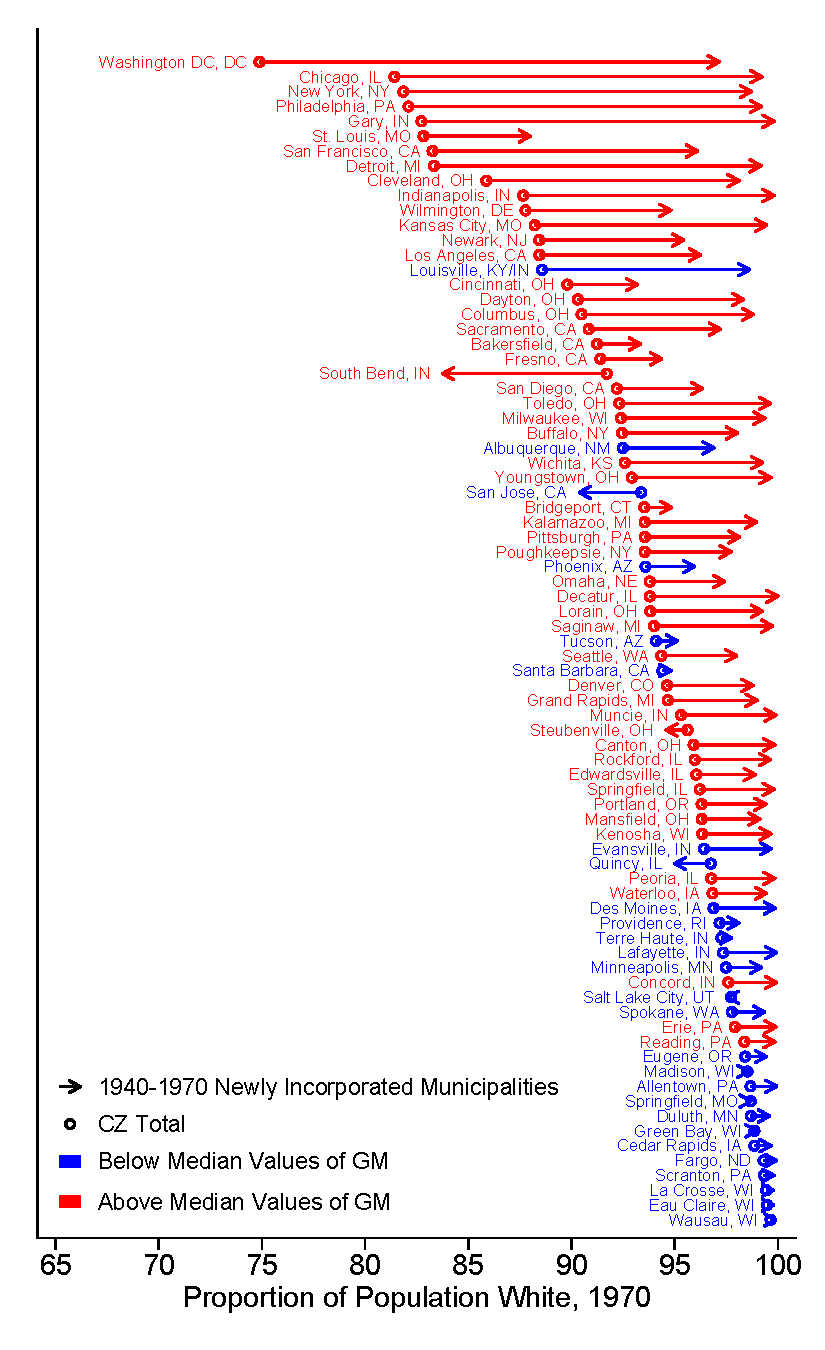
\includegraphics{figures/pcarrow_figure_GM.pdf}
\end{figure}
\clearpage
\begin{figure}
	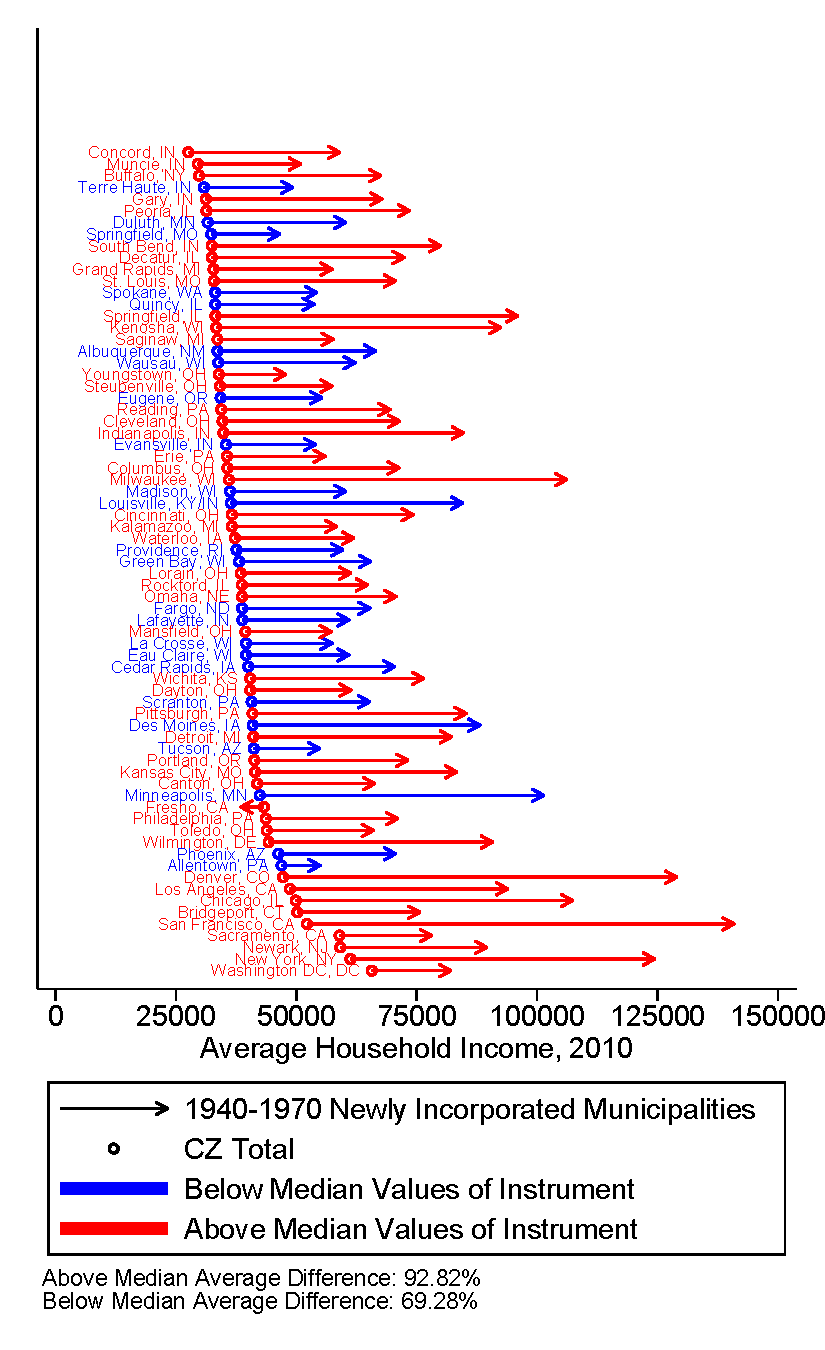
\includegraphics{figures/pcarrow_figure_inc2010.pdf}
\end{figure}
\clearpage
\begin{landscape}
\
\clearpage
\begin{tabular}{l*{10}{c}} \toprule
&\multicolumn{8}{l}{Panel A: Below Median GM CZs}\\
\cmidrule(lr){1-9}
&\multicolumn{2}{c}{1940-70 Incorporations}&\multicolumn{2}{c}{All other munis}&\multicolumn{2}{c}{Principle Cities}&\multicolumn{2}{c}{CZ Average}\\ \cmidrule(lr){2-3}  \cmidrule(lr){4-5} \cmidrule(lr){6-7} \cmidrule(lr){8-9}
                    &\multicolumn{2}{c}{}     &\multicolumn{2}{c}{}     &\multicolumn{2}{c}{}     &\multicolumn{2}{c}{}     \\
                    &        mean&          sd&        mean&          sd&        mean&          sd&        mean&          sd\\
\midrule
HH Income, 1970     &       12766&        3483&       10884&        1998&       10928&         961&       10249&        1208\\
Home Value, 1970    &    23926.41&     7993.26&    18911.51&     5168.46&    19071.57&     3848.10&    16704.70&     3683.49\\
HH Income, 2010     &    93106.92&    35914.21&    66251.96&    21733.07&    63186.18&    14829.39&    64193.71&    11133.63\\
Pct White, 1970     &       97.46&        4.58&       97.36&        3.03&       95.41&        2.47&       97.57&        2.38\\
Pct White, 2010     &       79.30&       17.70&       82.73&       14.06&       75.24&       14.12&       87.56&        8.02\\
 \toprule
&\multicolumn{8}{l}{Panel B: Above Median GM CZs}\\
\cmidrule(lr){1-9}
&\multicolumn{2}{c}{1940-70 Incorporations}&\multicolumn{2}{c}{All other munis}&\multicolumn{2}{c}{Principle Cities}&\multicolumn{2}{c}{CZ Average}\\ \cmidrule(lr){2-3}  \cmidrule(lr){4-5} \cmidrule(lr){6-7} \cmidrule(lr){8-9}
                    &\multicolumn{2}{c}{}     &\multicolumn{2}{c}{}     &\multicolumn{2}{c}{}     &\multicolumn{2}{c}{}     \\
                    &        mean&          sd&        mean&          sd&        mean&          sd&        mean&          sd\\
\midrule
HH Income, 1970     &       13909&        5272&       12744&        4930&       10899&         922&       11561&        1050\\
Home Value, 1970    &    24188.34&    10264.59&    19825.29&     9170.47&    17723.56&     4297.08&    19469.02&     4371.02\\
HH Income, 2010     &    85549.13&    50883.49&    72903.95&    41440.82&    52307.90&    14353.43&    68475.28&    12857.98\\
Pct White, 1970     &       96.50&       10.70&       96.63&        8.41&       79.97&       13.80&       92.06&        5.41\\
Pct White, 2010     &       80.14&       24.20&       89.44&       16.25&       59.45&       17.34&       79.32&       11.02\\
\toprule
&\multicolumn{8}{l}{Panel C: All CZs}\\
\cmidrule(lr){1-9}
&\multicolumn{2}{c}{1940-70 Incorporations}&\multicolumn{2}{c}{All other munis}&\multicolumn{2}{c}{Principle Cities}&\multicolumn{2}{c}{CZ Average}\\ \cmidrule(lr){2-3}  \cmidrule(lr){4-5} \cmidrule(lr){6-7} \cmidrule(lr){8-9}
                    &\multicolumn{2}{c}{}     &\multicolumn{2}{c}{}     &\multicolumn{2}{c}{}     &\multicolumn{2}{c}{}     \\
                    &        mean&          sd&        mean&          sd&        mean&          sd&        mean&          sd\\
\midrule
HH Income, 1970     &       13673&        5143&       12187&        4595&       10640&         980&        7041&        2498\\
Home Value, 1970    &    23466.38&    10127.76&    18463.10&     8568.00&    17379.00&     3989.75&    11080.05&     4545.15\\
HH Income, 2010     &    82269.09&    48062.29&    68406.05&    35778.02&    53366.29&    12657.06&    55682.89&     9825.92\\
Pct White, 1970     &       96.74&        9.62&       97.19&        7.41&       88.31&       12.97&       94.86&        4.97\\
Pct White, 2010     &       83.55&       21.74&       91.52&       14.13&       71.84&       18.86&       83.86&       10.64\\
\midrule \bottomrule \end{tabular}

\clearpage
\begin{figure}
	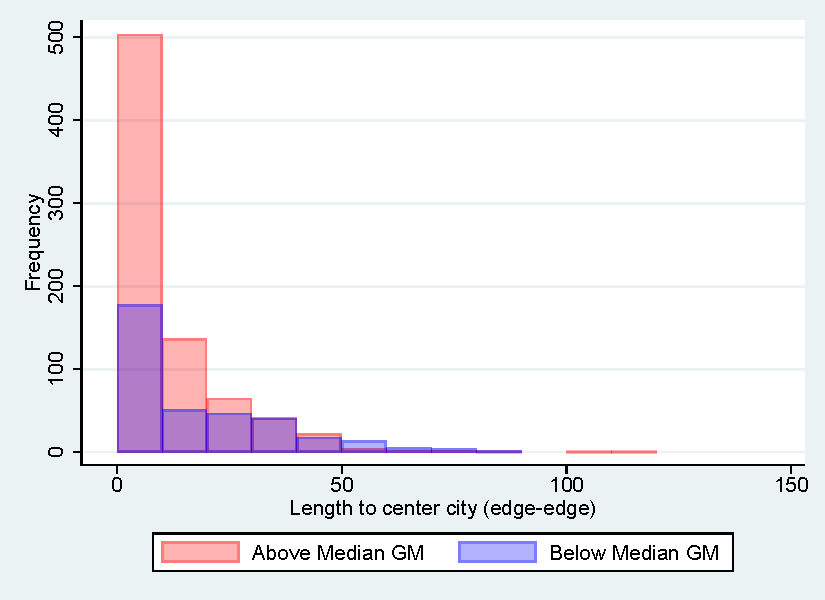
\includegraphics{figures/implications/dist_edge_edge_4070.pdf}
\end{figure}
\clearpage
\begin{figure}
	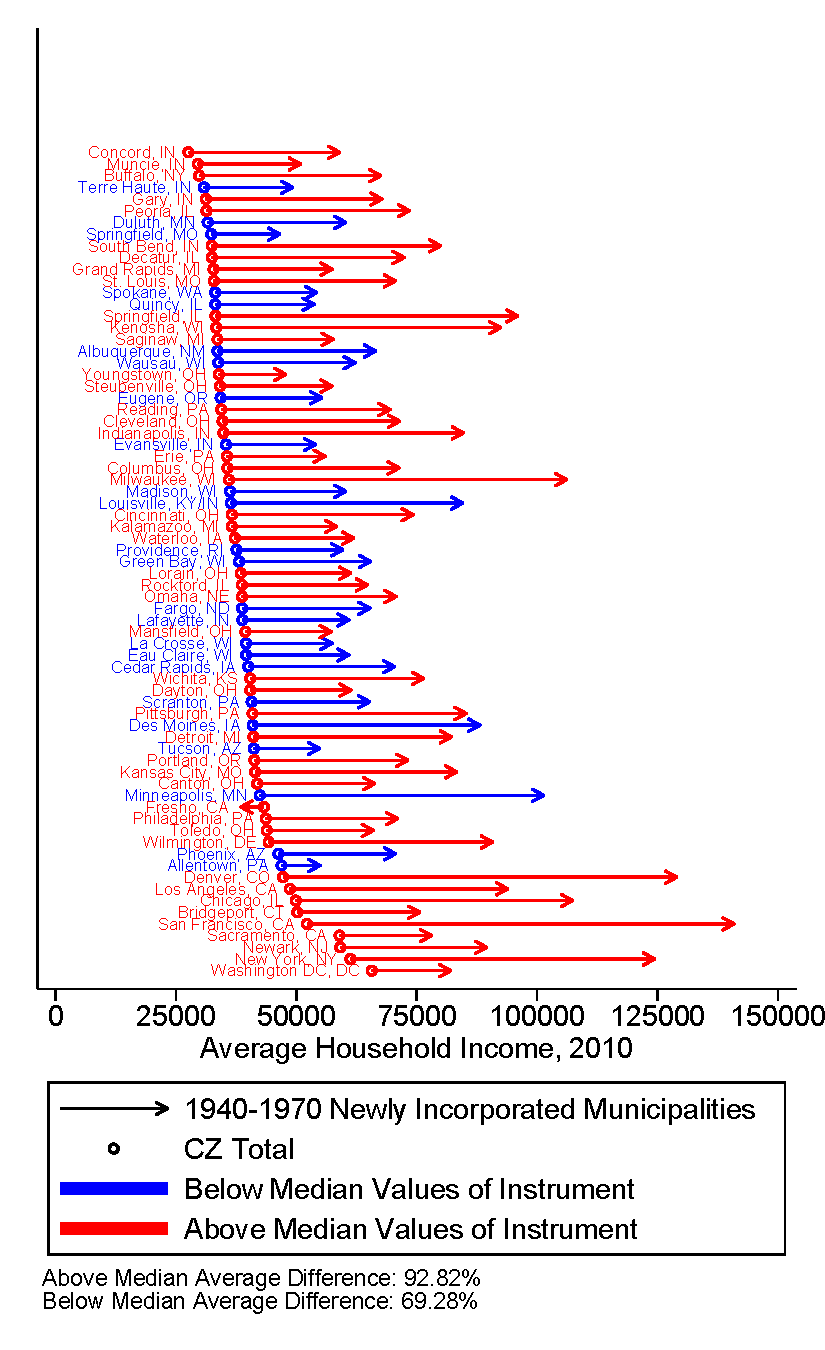
\includegraphics{figures/pcarrow_figure_inc2010.pdf}
\end{figure}
\clearpage
\begin{table}[htbp]\centering
\def\sym#1{\ifmmode^{#1}\else\(^{#1}\)\fi}
\caption{Economic Characteristics}
\begin{tabular}{l*{7}{c}}
\hline\hline
                    &\multicolumn{1}{c}{(1)}&\multicolumn{1}{c}{(2)}&\multicolumn{1}{c}{(3)}&\multicolumn{1}{c}{(4)}&\multicolumn{1}{c}{(5)}&\multicolumn{1}{c}{(6)}&\multicolumn{1}{c}{(7)}\\
                    &\multicolumn{1}{c}{Family Income, 1970}&\multicolumn{1}{c}{Home Value, 1970}&\multicolumn{1}{c}{Household Income, 2010}&\multicolumn{1}{c}{Prop White, 1970}&\multicolumn{1}{c}{Prop White, 2010}&\multicolumn{1}{c}{place\_pop1970}&\multicolumn{1}{c}{Muni Area}\\
\hline
Incorporated 1940-70&    1818.821         &   -1264.950         &    2427.757         &       8.302         &      12.626         &-3244843.865         &  -3.201e+07         \\
                    &  (1990.582)         &  (4979.257)         & (14611.107)         &     (5.095)         &     (9.044)         &(2017697.722)         &(50561626.426)         \\
[1em]
Above Median GM     &     827.587\sym{***}&    2152.461\sym{**} &    2302.127         &      -7.895\sym{***}&     -12.826\sym{***}&  347593.363         &-6268219.456         \\
                    &   (262.536)         &   (894.999)         &  (3416.881)         &     (0.994)         &     (3.085)         &(213280.006)         &(8120199.458)         \\
[1em]
Above Median GM X Inc. 1940-70&    -619.356         &   -2560.180\sym{***}&  -13240.523\sym{***}&       8.309\sym{***}&       9.336\sym{***}& -343132.011         &  -1.694e+07\sym{*}  \\
                    &   (500.678)         &   (969.601)         &  (4255.056)         &     (1.044)         &     (2.044)         &(214640.756)         &(8861990.259)         \\
\hline
Observations        &        2785         &        4251         &        7836         &        4343         &        7836         &        7849         &        7717         \\
\(R^{2}\)           &       0.104         &       0.261         &       0.132         &       0.260         &       0.269         &       0.290         &       0.337         \\
\hline\hline
\multicolumn{8}{l}{\footnotesize Standard errors in parentheses}\\
\multicolumn{8}{l}{\footnotesize \sym{*} \(p<0.10\), \sym{**} \(p<0.05\), \sym{***} \(p<0.01\)}\\
\end{tabular}
\end{table}

\clearpage

\begin{table}[htbp]\centering
\def\sym#1{\ifmmode^{#1}\else\(^{#1}\)\fi}
\caption{Raw Splits}
\begin{tabular}{l*{3}{c}}
\hline\hline
            &\multicolumn{1}{c}{(1)}&\multicolumn{1}{c}{(2)}&\multicolumn{1}{c}{(3)}\\
            &\multicolumn{1}{c}{touching}&\multicolumn{1}{c}{below\_len\_edge}&\multicolumn{1}{c}{len\_edge\_edge}\\
\hline
samp\_dest   &       0.095         &      -0.109         &      -1.050         \\
            &     (0.312)         &     (0.242)         &     (8.510)         \\
[1em]
above\_x\_med &      -0.041         &      -0.040         &       0.465         \\
            &     (0.058)         &     (0.055)         &     (2.342)         \\
[1em]
samp\_destXabove\_x\_med&       0.021         &      -0.023         &       1.852         \\
            &     (0.160)         &     (0.048)         &     (1.927)         \\
\hline
\(N\)       &        8514         &        8514         &        8386         \\
\(R^{2}\)   &       0.038         &       0.072         &       0.085         \\
\hline\hline
\multicolumn{4}{l}{\footnotesize Standard errors in parentheses}\\
\multicolumn{4}{l}{\footnotesize \sym{*} \(p<0.10\), \sym{**} \(p<0.05\), \sym{***} \(p<0.01\)}\\
\end{tabular}
\end{table}

\clearpage
\begin{table}[htbp]\centering
\def\sym#1{\ifmmode^{#1}\else\(^{#1}\)\fi}
\caption{Raw Splits}
\begin{tabular}{l*{4}{c}}
\hline\hline
            &\multicolumn{1}{c}{(1)}&\multicolumn{1}{c}{(2)}&\multicolumn{1}{c}{(3)}&\multicolumn{1}{c}{(4)}\\
            &\multicolumn{1}{c}{exclusive\_district\_place}&\multicolumn{1}{c}{exclusive\_district\_shape}&\multicolumn{1}{c}{psum\_shared\_boundary\_muni}&\multicolumn{1}{c}{min\_hausdorff\_muni}\\
\hline
samp\_dest   &      -0.972\sym{***}&       0.417         &       0.082         &      -0.070\sym{*}  \\
            &     (0.341)         &     (0.287)         &     (0.190)         &     (0.037)         \\
[1em]
above\_x\_med &      -0.042         &      -0.309\sym{*}  &       0.068         &      -0.005         \\
            &     (0.069)         &     (0.166)         &     (0.044)         &     (0.011)         \\
[1em]
samp\_destXabove\_x\_med&       0.209\sym{***}&       0.403\sym{**} &       0.030         &      -0.020\sym{*}  \\
            &     (0.077)         &     (0.167)         &     (0.065)         &     (0.011)         \\
\hline
\(N\)       &        8836         &        8836         &        8836         &        8836         \\
\(R^{2}\)   &       0.163         &       0.480         &       0.166         &       0.446         \\
\hline\hline
\multicolumn{5}{l}{\footnotesize Standard errors in parentheses}\\
\multicolumn{5}{l}{\footnotesize \sym{*} \(p<0.10\), \sym{**} \(p<0.05\), \sym{***} \(p<0.01\)}\\
\end{tabular}
\end{table}

\clearpage

\begin{table}[htbp]\centering
\def\sym#1{\ifmmode^{#1}\else\(^{#1}\)\fi}
\caption{Raw Splits}
\begin{tabular}{l*{5}{c}}
\hline\hline
            &\multicolumn{1}{c}{(1)}&\multicolumn{1}{c}{(2)}&\multicolumn{1}{c}{(3)}&\multicolumn{1}{c}{(4)}&\multicolumn{1}{c}{(5)}\\
            &\multicolumn{1}{c}{landuse\_sfr}&\multicolumn{1}{c}{landuse\_apartment}&\multicolumn{1}{c}{pct\_rev\_ff}&\multicolumn{1}{c}{pct\_rev\_sa}&\multicolumn{1}{c}{pct\_rev\_debt}\\
\hline
samp\_dest   &      27.137\sym{**} &      -2.910\sym{***}&       0.018         &       0.809         &      92.093         \\
            &    (11.206)         &     (0.779)         &     (1.078)         &     (1.173)         &   (175.905)         \\
[1em]
above\_x\_med &      -0.751         &       0.619\sym{**} &       0.391\sym{***}&       0.473         &     -61.021\sym{*}  \\
            &     (2.532)         &     (0.270)         &     (0.138)         &     (0.419)         &    (33.267)         \\
[1em]
samp\_destXabove\_x\_med&      10.255\sym{***}&      -0.731\sym{***}&       0.707\sym{**} &      -2.074\sym{***}&      40.542         \\
            &     (2.933)         &     (0.231)         &     (0.309)         &     (0.566)         &    (52.894)         \\
\hline
\(N\)       &        8699         &        8699         &        8694         &        8694         &        8694         \\
\(R^{2}\)   &       0.791         &       0.785         &       0.158         &       0.117         &       0.207         \\
\hline\hline
\multicolumn{6}{l}{\footnotesize Standard errors in parentheses}\\
\multicolumn{6}{l}{\footnotesize \sym{*} \(p<0.10\), \sym{**} \(p<0.05\), \sym{***} \(p<0.01\)}\\
\end{tabular}
\end{table}

\clearpage
\begin{table}[htbp]\centering
\def\sym#1{\ifmmode^{#1}\else\(^{#1}\)\fi}
\caption{Raw Splits}
\begin{tabular}{l*{7}{c}}
\hline\hline
            &\multicolumn{1}{c}{(1)}&\multicolumn{1}{c}{(2)}&\multicolumn{1}{c}{(3)}&\multicolumn{1}{c}{(4)}&\multicolumn{1}{c}{(5)}&\multicolumn{1}{c}{(6)}&\multicolumn{1}{c}{(7)}\\
            &\multicolumn{1}{c}{mf}&\multicolumn{1}{c}{mixed\_use}&\multicolumn{1}{c}{attached\_sfr}&\multicolumn{1}{c}{adu}&\multicolumn{1}{c}{flex\_zoning\_br}&\multicolumn{1}{c}{min\_lot\_size\_mean}&\multicolumn{1}{c}{min\_lot\_size\_max}\\
\hline
samp\_dest   &      -0.094         &      -0.831         &      -0.760\sym{***}&      -1.184\sym{**} &      -0.154         &   49889.752\sym{**} &  139634.815         \\
            &     (0.082)         &     (0.557)         &     (0.196)         &     (0.596)         &     (0.248)         & (23167.306)         & (84248.118)         \\
[1em]
above\_x\_med &      -0.000         &      -0.128\sym{***}&       0.384\sym{***}&       0.093         &       0.189         &   -7415.561         &  -53398.490\sym{*}  \\
            &     (0.004)         &     (0.040)         &     (0.130)         &     (0.125)         &     (0.136)         &  (6868.233)         & (31694.361)         \\
[1em]
samp\_destXabove\_x\_med&       0.002         &       0.037         &      -0.411\sym{***}&      -0.228\sym{*}  &      -0.227         &   -2933.187         &   46993.519         \\
            &     (0.008)         &     (0.090)         &     (0.096)         &     (0.137)         &     (0.163)         &  (9744.735)         & (33741.665)         \\
\hline
\(N\)       &        3349         &        3326         &        3401         &        3383         &        3402         &        3156         &        3150         \\
\(R^{2}\)   &       0.008         &       0.086         &       0.382         &       0.321         &       0.192         &       0.228         &       0.230         \\
\hline\hline
\multicolumn{8}{l}{\footnotesize Standard errors in parentheses}\\
\multicolumn{8}{l}{\footnotesize \sym{*} \(p<0.10\), \sym{**} \(p<0.05\), \sym{***} \(p<0.01\)}\\
\end{tabular}
\end{table}

\clearpage
\begin{table}[htbp]\centering
\def\sym#1{\ifmmode^{#1}\else\(^{#1}\)\fi}
\caption{AI Zoning - Regulations}
\begin{tabular}{l*{5}{c}}
\hline\hline
                    &\multicolumn{1}{c}{(1)}&\multicolumn{1}{c}{(2)}&\multicolumn{1}{c}{(3)}&\multicolumn{1}{c}{(4)}&\multicolumn{1}{c}{(5)}\\
                    &\multicolumn{1}{c}{Inclusionary Zoning}&\multicolumn{1}{c}{Permit caps}&\multicolumn{1}{c}{Number of agencies}&\multicolumn{1}{c}{Public hearings for MF}&\multicolumn{1}{c}{Max review days}\\
\hline
Incorporated 1940-70&       0.301         &       0.903\sym{***}&      -1.248\sym{*}  &       0.601\sym{*}  &     -82.383         \\
                    &     (0.356)         &     (0.299)         &     (0.644)         &     (0.334)         &    (93.938)         \\
[1em]
Above Median GM     &       0.179\sym{*}  &       0.004         &      -0.194         &       0.130         &      68.079\sym{***}\\
                    &     (0.106)         &     (0.059)         &     (0.159)         &     (0.085)         &    (22.275)         \\
[1em]
Above Median GM X Inc. 1940-70&      -0.502\sym{***}&      -0.005         &       0.963\sym{***}&      -0.083         &     -34.216         \\
                    &     (0.089)         &     (0.060)         &     (0.222)         &     (0.102)         &    (31.136)         \\
\hline
Observations        &        2520         &        2637         &        2613         &        2599         &        2311         \\
\(R^{2}\)           &       0.215         &       0.047         &       0.068         &       0.048         &       0.108         \\
\hline\hline
\multicolumn{6}{l}{\footnotesize Standard errors in parentheses}\\
\multicolumn{6}{l}{\footnotesize \sym{*} \(p<0.10\), \sym{**} \(p<0.05\), \sym{***} \(p<0.01\)}\\
\end{tabular}
\end{table}

\clearpage

\begin{table}[htbp]\centering
\def\sym#1{\ifmmode^{#1}\else\(^{#1}\)\fi}
\caption{Muni-District similarity, CZ level}
\begin{tabular}{l*{4}{c}}
\hline\hline
            &\multicolumn{1}{c}{(1)}&\multicolumn{1}{c}{(2)}&\multicolumn{1}{c}{(3)}&\multicolumn{1}{c}{(4)}\\
            &\multicolumn{1}{c}{EI}&\multicolumn{1}{c}{mean\_dist\_max\_int}&\multicolumn{1}{c}{mean\_min\_hausdorff\_muni}&\multicolumn{1}{c}{mean\_psum\_shared\_muni}\\
\hline
GM\_raw\_pp   &       0.007\sym{***}&       0.011\sym{***}&      -0.004\sym{***}&       0.005         \\
            &     (0.003)         &     (0.003)         &     (0.001)         &     (0.004)         \\
\hline
\(N\)       &         118         &         118         &         118         &         118         \\
\(R^{2}\)   &       0.681         &       0.709         &       0.742         &       0.342         \\
\hline\hline
\multicolumn{5}{l}{\footnotesize Standard errors in parentheses}\\
\multicolumn{5}{l}{\footnotesize \sym{*} \(p<0.10\), \sym{**} \(p<0.05\), \sym{***} \(p<0.01\)}\\
\end{tabular}
\end{table}

\clearpage
\begin{table}[htbp]\centering
\def\sym#1{\ifmmode^{#1}\else\(^{#1}\)\fi}
\caption{Raw Splits}
\begin{tabular}{l*{4}{c}}
\hline\hline
            &\multicolumn{1}{c}{(1)}&\multicolumn{1}{c}{(2)}&\multicolumn{1}{c}{(3)}&\multicolumn{1}{c}{(4)}\\
            &\multicolumn{1}{c}{vr\_blwt\_cz}&\multicolumn{1}{c}{diss\_blwt\_cz}&\multicolumn{1}{c}{SP\_nexpd\_1970}&\multicolumn{1}{c}{rco1970}\\
\hline
GM\_raw\_pp   &       0.016\sym{***}&       0.003\sym{***}&       0.007\sym{***}&      -0.033\sym{***}\\
            &     (0.003)         &     (0.001)         &     (0.002)         &     (0.007)         \\
\hline
\(N\)       &         118         &         118         &         130         &         130         \\
\(R^{2}\)   &       0.724         &       0.582         &       0.258         &       0.433         \\
\hline\hline
\multicolumn{5}{l}{\footnotesize Standard errors in parentheses}\\
\multicolumn{5}{l}{\footnotesize \sym{*} \(p<0.10\), \sym{**} \(p<0.05\), \sym{***} \(p<0.01\)}\\
\end{tabular}
\end{table}

\clearpage
\begin{table}[htbp]\centering
\def\sym#1{\ifmmode^{#1}\else\(^{#1}\)\fi}
\caption{School District Amenities}
\begin{tabular}{l*{5}{c}}
\hline\hline
            &\multicolumn{1}{c}{(1)}&\multicolumn{1}{c}{(2)}&\multicolumn{1}{c}{(3)}&\multicolumn{1}{c}{(4)}&\multicolumn{1}{c}{(5)}\\
            &\multicolumn{1}{c}{mean\_ap}&\multicolumn{1}{c}{totenroll}&\multicolumn{1}{c}{st\_ratio\_leaid}&\multicolumn{1}{c}{pct\_white\_leaid}&\multicolumn{1}{c}{pct\_free\_red\_lunch\_leaid}\\
\hline
int\_0       &      35.346         &    5567.768\sym{*}  &      15.801         &      -2.097\sym{***}&       0.711         \\
            &    (22.336)         &  (3010.331)         &    (12.475)         &     (0.519)         &     (0.708)         \\
[1em]
above\_x\_med &       1.177         &     193.388\sym{**} &       1.910\sym{***}&      -0.087\sym{**} &       0.010         \\
            &     (0.925)         &    (78.164)         &     (0.474)         &     (0.037)         &     (0.022)         \\
[1em]
above\_x\_med\_int\_0&      -4.696         &    -872.194\sym{***}&      -3.359\sym{**} &       0.233\sym{***}&       0.045         \\
            &     (3.479)         &   (324.655)         &     (1.512)         &     (0.074)         &     (0.127)         \\
[1em]
above\_x\_med\_int\_0&       0.000         &       0.000         &       0.000         &       0.000         &       0.000         \\
            &         (.)         &         (.)         &         (.)         &         (.)         &         (.)         \\
\hline
\(N\)       &        3089         &        4224         &        4199         &        4224         &        4224         \\
\(R^{2}\)   &       0.118         &       0.081         &       0.395         &       0.369         &       0.082         \\
\hline\hline
\multicolumn{6}{l}{\footnotesize Standard errors in parentheses}\\
\multicolumn{6}{l}{\footnotesize \sym{*} \(p<0.10\), \sym{**} \(p<0.05\), \sym{***} \(p<0.01\)}\\
\end{tabular}
\end{table}

\clearpage
 \begin{tabular}{l*{9}{c}} \toprule
&\multicolumn{1}{c}{All}&\multicolumn{1}{c}{White}&\multicolumn{1}{c}{Black}&\multicolumn{1}{c}{W-B Gap}&\multicolumn{1}{c}{Not Ec. Disadvantaged}&\multicolumn{1}{c}{Ec. Disadvantaged}&\multicolumn{1}{c}{NEC-ECD Gap}&\\\cmidrule(lr){2-2}\cmidrule(lr){3-3}\cmidrule(lr){4-4}\cmidrule(lr){5-5}\cmidrule(lr){6-6}\cmidrule(lr){7-7}\cmidrule(lr){8-8}
&\multicolumn{1}{c}{(1)}&\multicolumn{1}{c}{(2)}&\multicolumn{1}{c}{(3)}&\multicolumn{1}{c}{(4)}&\multicolumn{1}{c}{(5)}&\multicolumn{1}{c}{(6)}&\multicolumn{1}{c}{(7)}\\
\cmidrule(lr){1-8}
\multicolumn{7}{l}{Panel A: IV with GM}\\
\cmidrule(lr){1-8}
Percentage Point Change in Urban Black Population&   -0.003   &    0.002   &   -0.001   &    0.003   &   -0.002   &   -0.003** &    0.001   \\
                &  (0.002)   &  (0.004)   &  (0.002)   &  (0.003)   &  (0.002)   &  (0.001)   &  (0.002)   \\
\cmidrule(lr){1-8}
\multicolumn{7}{l}{Panel B: OLS with Munis}\\
\cmidrule(lr){1-8}
New Number of Municipal Govts, P.C. (total)&   -0.114** &    0.083   &   -0.010   &    0.079   &    0.010   &   -0.040   &    0.046   \\
                &  (0.047)   &  (0.077)   &  (0.039)   &  (0.072)   &  (0.049)   &  (0.037)   &  (0.054)   \\
\cmidrule(lr){1-8}
\multicolumn{7}{l}{Panel C: Two Step with Munis}\\
\cmidrule(lr){1-8}
New Number of Municipal Govts, P.C. (total)&   -0.493** &   -0.098   &   -0.404** &    0.244   &   -0.454** &   -0.498***&    0.032   \\
                &  (0.198)   &  (0.333)   &  (0.156)   &  (0.246)   &  (0.213)   &  (0.131)   &  (0.168)   \\
\midrule
Dep. Var Mean   &    0.045   &    0.180   &   -0.377   &    0.562   &    0.318   &   -0.255   &    0.574   \\
Observations    &      130   &      130   &      130   &      130   &      130   &      130   &      130   \\
\cmidrule(lr){1-8}
\multicolumn{7}{l}{Panel B: OLS with School Districts}\\
\cmidrule(lr){1-8}
New Ind. Sch. Dists., P.C. (total)&    0.001   &    0.006***&    0.003** &    0.002   &    0.002*  &    0.001   &    0.001   \\
                &  (0.002)   &  (0.002)   &  (0.001)   &  (0.002)   &  (0.001)   &  (0.001)   &  (0.002)   \\
\cmidrule(lr){1-8}
\multicolumn{7}{l}{Panel E: Two Step with School Districts}\\
\cmidrule(lr){1-8}
New Ind. Sch. Dists., P.C. (total)&   -0.005** &   -0.001   &   -0.004** &    0.001   &   -0.007** &   -0.007***&   -0.001   \\
                &  (0.003)   &  (0.005)   &  (0.002)   &  (0.005)   &  (0.003)   &  (0.002)   &  (0.003)   \\
\midrule
Dep. Var Mean   &    0.039   &    0.174   &   -0.390   &    0.570   &    0.313   &   -0.258   &    0.572   \\
Observations    &      118   &      118   &      118   &      118   &      118   &      118   &      118   \\
       \bottomrule \end{tabular}

\clearpage
\begin{table}[htbp]\centering
\def\sym#1{\ifmmode^{#1}\else\(^{#1}\)\fi}
\caption{School District Capital Expenditure}
\begin{tabular}{l*{4}{c}}
\hline\hline
                    &\multicolumn{1}{c}{(1)}&\multicolumn{1}{c}{(2)}&\multicolumn{1}{c}{(3)}&\multicolumn{1}{c}{(4)}\\
                    &\multicolumn{1}{c}{Capital outlays/Total Expenditure}&\multicolumn{1}{c}{Capital outlays/Total Enrollment}&\multicolumn{1}{c}{Log Capital Outlays}&\multicolumn{1}{c}{log(Capital outlays/Total Enrollment)}\\
\hline
Prop Border with 40-70 incorporation&       0.040         &       1.275         &       2.175         &       1.288         \\
                    &     (0.088)         &  (1318.729)         &     (2.454)         &     (1.254)         \\
[1em]
Above Median GM     &      -0.002         &      73.278         &       0.516\sym{**} &       0.137         \\
                    &     (0.009)         &   (105.966)         &     (0.214)         &     (0.104)         \\
[1em]
Prop Border 40-70 X Above Median GM&      -0.036         &    -385.582         &      -1.882\sym{***}&      -0.520\sym{**} \\
                    &     (0.022)         &   (364.857)         &     (0.496)         &     (0.244)         \\
\hline
Observations        &        4117         &        4117         &        4116         &        4116         \\
\(R^{2}\)           &       0.063         &       0.013         &       0.180         &       0.055         \\
\hline\hline
\multicolumn{5}{l}{\footnotesize Standard errors in parentheses}\\
\multicolumn{5}{l}{\footnotesize \sym{*} \(p<0.10\), \sym{**} \(p<0.05\), \sym{***} \(p<0.01\)}\\
\end{tabular}
\end{table}

\clearpage

\begin{tabular}{l*{7}{c}} \toprule
&\multicolumn{2}{c}{School District Segregation}&\multicolumn{4}{c}{School District Achievement}\\\cmidrule(lr){2-3}\cmidrule(lr){4-7}
&\multicolumn{1}{c}{\shortstack{Variance \\ Ratio}}&\multicolumn{1}{c}{\shortstack{Dissimilarity \\ Index}}&\multicolumn{1}{c}{\shortstack{Interquartile \\ Range}}&\multicolumn{1}{c}{\shortstack{Variance}}&\multicolumn{1}{c}{\shortstack{Black}}&\multicolumn{1}{c}{\shortstack{White}}\\\cmidrule(lr){2-2}\cmidrule(lr){3-3}\cmidrule(lr){4-4}\cmidrule(lr){5-5}\cmidrule(lr){6-6}\cmidrule(lr){7-7}
&\multicolumn{1}{c}{(1)}&\multicolumn{1}{c}{(2)}&\multicolumn{1}{c}{(3)}&\multicolumn{1}{c}{(4)}&\multicolumn{1}{c}{(5)}&\multicolumn{1}{c}{(6)}\\
\cmidrule(lr){1-7}
\multicolumn{6}{l}{Panel A: First Stage}\\
\cmidrule(lr){1-7}
Predicted Percentage Change in Urban Black Population&    1.341***&    1.341***&    1.341***&    1.341***&    1.341***&    1.341***\\
                &  (0.377)   &  (0.377)   &  (0.377)   &  (0.377)   &  (0.377)   &  (0.377)   \\
\cmidrule(lr){1-7}
\multicolumn{6}{l}{Panel B: OLS}\\
\cmidrule(lr){1-7}
$\Delta\_{1940-70}$ School Districts P.C.&    0.012***&    0.003***&    0.009***&    0.004***&   -0.005** &    0.006***\\
                &  (0.002)   &  (0.001)   &  (0.002)   &  (0.001)   &  (0.002)   &  (0.001)   \\
\cmidrule(lr){1-7}
\multicolumn{6}{l}{Panel C: Reduced Form}\\
\cmidrule(lr){1-7}
Predicted Percentage Change in Urban Black Population&    0.037***&    0.008***&    0.022** &    0.010***&   -0.021** &   -0.021** \\
                &  (0.007)   &  (0.002)   &  (0.010)   &  (0.004)   &  (0.008)   &  (0.008)   \\
\cmidrule(lr){1-7}
\multicolumn{6}{l}{Panel D: 2SLS}\\
\cmidrule(lr){1-7}
$\Delta\_{1940-70}$ School Districts P.C.&    0.027***&    0.006***&    0.016***&    0.008***&   -0.016** &    0.000   \\
                &  (0.005)   &  (0.001)   &  (0.004)   &  (0.001)   &  (0.007)   &  (0.004)   \\
\midrule
First Stage F-Stat&    12.67   &    12.67   &    12.67   &    12.67   &    12.67   &    12.67   \\
Dep. Var. Mean  &     0.21   &     0.26   &     0.32   &     0.07   &    -0.13   &     0.11   \\
Observations    &      118   &      118   &      118   &      118   &      118   &      118   \\
 \bottomrule \end{tabular}

\clearpage

 \begin{tabular}{l*{9}{c}} \toprule
&\multicolumn{1}{c}{VR}&\multicolumn{1}{c}{Diss}&\multicolumn{1}{c}{RCO}&\multicolumn{1}{c}{SP}&\multicolumn{1}{c}{Atkinson ($\beta = 0.1$)}&\multicolumn{1}{c}{Atkinson ($\beta - 0.9$)}\\\cmidrule(lr){2-2}\cmidrule(lr){3-3}\cmidrule(lr){4-4}\cmidrule(lr){5-5}\cmidrule(lr){6-6}\cmidrule(lr){7-7}
&\multicolumn{1}{c}{(1)}&\multicolumn{1}{c}{(2)}&\multicolumn{1}{c}{(3)}&\multicolumn{1}{c}{(4)}&\multicolumn{1}{c}{(5)}&\multicolumn{1}{c}{(6)}\\
\cmidrule(lr){1-7}
\multicolumn{6}{l}{Panel A: IV with GM}\\
\cmidrule(lr){1-7}
Percentage Point Change in Urban Black Population&    0.012***&    0.003***&   -0.037*  &    0.016** &    0.002***&    0.012***\\
                &  (0.002)   &  (0.001)   &  (0.023)   &  (0.008)   &  (0.001)   &  (0.003)   \\
\cmidrule(lr){1-7}
\multicolumn{6}{l}{Panel B: OLS with Munis}\\
\cmidrule(lr){1-7}
New Number of Municipal Govts, P.C. (total)&    0.111*  &    0.017   &   -0.345   &    0.071   &    0.011   &    0.101   \\
                &  (0.067)   &  (0.040)   &  (0.296)   &  (0.156)   &  (0.018)   &  (0.098)   \\
\cmidrule(lr){1-7}
\multicolumn{6}{l}{Panel C: Two Step with Munis}\\
\cmidrule(lr){1-7}
New Number of Municipal Govts, P.C. (total)&    1.387***&    0.501***&   -4.764** &    2.086** &    0.260***&    1.484***\\
                &  (0.208)   &  (0.089)   &  (2.059)   &  (0.807)   &  (0.042)   &  (0.204)   \\
\midrule
Dep. Var Mean   &    0.092   &    0.192   &   -0.496   &    1.112   &    0.080   &    0.340   \\
Observations    &      130   &      130   &      130   &      130   &      130   &      130   \\
\cmidrule(lr){1-7}
\multicolumn{6}{l}{Panel D: OLS with School Districts}\\
\cmidrule(lr){1-7}
New Ind. Sch. Dists., P.C. (total)&    0.009***&    0.004***&   -0.031***&    0.012** &    0.001***&    0.011***\\
                &  (0.002)   &  (0.001)   &  (0.010)   &  (0.005)   &  (0.000)   &  (0.002)   \\
\cmidrule(lr){1-7}
\multicolumn{6}{l}{Panel E: Two Step with School Districts}\\
\cmidrule(lr){1-7}
New Ind. Sch. Dists., P.C. (total)&    0.029***&    0.012***&   -0.101** &    0.045***&    0.005***&    0.033***\\
                &  (0.004)   &  (0.002)   &  (0.039)   &  (0.015)   &  (0.001)   &  (0.004)   \\
\midrule
Dep. Var Mean   &    0.093   &    0.194   &   -0.529   &    1.115   &    0.083   &    0.348   \\
Observations    &      118   &      118   &      118   &      118   &      118   &      118   \\
       \bottomrule \end{tabular}

\clearpage

 \begin{tabular}{l*{7}{c}} \toprule
                &\multicolumn{1}{c}{(1)}&\multicolumn{1}{c}{(2)}&\multicolumn{1}{c}{(3)}&\multicolumn{1}{c}{(4)}&\multicolumn{1}{c}{(5)}&\multicolumn{1}{c}{(6)}\\
                &\multicolumn{1}{c}{\shortstack{Variance \\ Ratio}}&\multicolumn{1}{c}{\shortstack{Dissimilarity \\ Index}}&\multicolumn{1}{c}{\shortstack{Relative \\ Concentration}}&\multicolumn{1}{c}{\shortstack{Spatial \\ Proximity}}&\multicolumn{1}{c}{\shortstack{Atkinson \\ Index ($\beta = 0.1$)}}&\multicolumn{1}{c}{\shortstack{Atkinson \\ Index ($\beta = 0.9$)}}\\
\cmidrule(lr){1-7}
\multicolumn{6}{l}{Panel A: IV with GM}\\
\cmidrule(lr){1-7}
GM              &    0.015***&    0.003***&   -0.026   &    0.015***&    0.002***&    0.012***\\
                &  (0.002)   &  (0.001)   &  (0.026)   &  (0.006)   &  (0.000)   &  (0.002)   \\
\cmidrule(lr){1-7}
\multicolumn{6}{l}{Panel B: OLS with $\Delta$ School Districts Per Capita}\\
\cmidrule(lr){1-7}
$\Delta$ School Districts P.C.&    0.012***&    0.003***&   -0.032   &    0.016***&    0.002***&    0.011***\\
                &  (0.002)   &  (0.001)   &  (0.021)   &  (0.004)   &  (0.000)   &  (0.002)   \\
\midrule
Dep. Var. Mean  &    0.092   &    0.192   &   -0.496   &    1.112   &    0.114   &    0.549   \\
Observations    &      118   &      118   &      118   &      118   &      118   &      118   \\
      \bottomrule \end{tabular}

\clearpage

\clearpage
 \begin{tabular}{l*{8}{c}} \toprule
&\multicolumn{1}{c}{C. Goodman}&\multicolumn{4}{c}{Census of Governments}&\multicolumn{1}{c}{Census}\\\cmidrule(lr){2-2}\cmidrule(lr){3-6}\cmidrule(lr){7-7}
&\multicolumn{2}{c}{Municipalities}&\multicolumn{1}{c}{School districts}&\multicolumn{1}{c}{Townships}&\multicolumn{1}{c}{Special districts}&\multicolumn{1}{c}{Principal City Share}\\\cmidrule(lr){2-3}\cmidrule(lr){4-6}\cmidrule(lr){7-7}
&\multicolumn{1}{c}{(1)}&\multicolumn{1}{c}{(2)}&\multicolumn{1}{c}{(3)}&\multicolumn{1}{c}{(4)}&\multicolumn{1}{c}{(5)}&\multicolumn{1}{c}{(6)}\\
\cmidrule(lr){1-7}
\multicolumn{6}{l}{Panel A: First Stage}\\
\cmidrule(lr){1-7}
$\widehat{GM}$  &    2.263***&    2.263***&    2.263***&    2.263***&    2.263***&    2.263***\\
                &  (0.457)   &  (0.457)   &  (0.457)   &  (0.457)   &  (0.457)   &  (0.457)   \\
\cmidrule(lr){1-7}
\multicolumn{6}{l}{Panel B: OLS}\\
\cmidrule(lr){1-7}
GM              &    0.002   &    0.005   &   -0.046   &    0.009   &   -0.035***&   -1.063***\\
                &  (0.003)   &  (0.004)   &  (0.076)   &  (0.006)   &  (0.009)   &  (0.144)   \\
\cmidrule(lr){1-7}
\multicolumn{6}{l}{Panel C: Reduced Form}\\
\cmidrule(lr){1-7}
$\widehat{GM}$  &    0.028*  &    0.042** &    0.465   &    0.084***&   -0.066*  &   -4.229***\\
                &  (0.016)   &  (0.018)   &  (0.424)   &  (0.032)   &  (0.037)   &  (0.726)   \\
\cmidrule(lr){1-7}
\multicolumn{6}{l}{Panel D: 2SLS}\\
\cmidrule(lr){1-7}
GM              &    0.013*  &    0.018** &    0.206   &    0.037** &   -0.029*  &   -1.869***\\
                &  (0.007)   &  (0.008)   &  (0.188)   &  (0.015)   &  (0.016)   &  (0.243)   \\
\midrule
First Stage F-Stat&    24.48   &    24.48   &    24.48   &    24.48   &    24.48   &    24.48   \\
Dependent Variable Mean&     -.14   &     -.17   &    -3.57   &     -.25   &      .26   &   -14.64   \\
Observations    &      130   &      130   &      130   &      130   &      130   &      130   \\
       \bottomrule \end{tabular}

\clearpage
 \begin{tabular}{l*{8}{c}} \toprule
&\multicolumn{1}{c}{C. Goodman}&\multicolumn{4}{c}{Census of Governments}&\multicolumn{1}{c}{Census}\\\cmidrule(lr){2-2}\cmidrule(lr){3-6}\cmidrule(lr){7-7}
&\multicolumn{2}{c}{Municipalities}&\multicolumn{1}{c}{School districts}&\multicolumn{1}{c}{Townships}&\multicolumn{1}{c}{Special districts}&\multicolumn{1}{c}{Main City Share}\\\cmidrule(lr){2-3}\cmidrule(lr){4-6}\cmidrule(lr){7-7}
&\multicolumn{1}{c}{(1)}&\multicolumn{1}{c}{(2)}&\multicolumn{1}{c}{(3)}&\multicolumn{1}{c}{(4)}&\multicolumn{1}{c}{(5)}&\multicolumn{1}{c}{(6)}\\
\cmidrule(lr){1-7}
\multicolumn{6}{l}{Panel A: First Stage}\\
\cmidrule(lr){1-7}
$\widehat{GM}$  &    2.185***&    2.185***&    2.185***&    2.185***&    2.185***&    2.185***\\
                &  (0.302)   &  (0.302)   &  (0.302)   &  (0.302)   &  (0.302)   &  (0.302)   \\
\cmidrule(lr){1-7}
\multicolumn{6}{l}{Panel B: OLS}\\
\cmidrule(lr){1-7}
GM              &    0.010   &    0.016** &    1.084***&    0.013   &   -0.073***&   -1.029***\\
                &  (0.006)   &  (0.007)   &  (0.293)   &  (0.011)   &  (0.016)   &  (0.237)   \\
\addlinespace
GM\_raw\_pp\_2     &   -0.000   &   -0.000   &   -0.024** &    0.000   &    0.002***&    0.004   \\
                &  (0.000)   &  (0.000)   &  (0.009)   &  (0.000)   &  (0.000)   &  (0.006)   \\
\cmidrule(lr){1-7}
\multicolumn{6}{l}{Panel C: Reduced Form}\\
\cmidrule(lr){1-7}
$\widehat{GM}$  &    0.047***&    0.059***&    3.306***&    0.100***&   -0.127***&   -4.316***\\
                &  (0.012)   &  (0.012)   &  (0.588)   &  (0.024)   &  (0.033)   &  (0.649)   \\
\addlinespace
GM\_hat\_raw\_2    &   -0.002***&   -0.003***&   -0.210***&   -0.003***&    0.005***&    0.129***\\
                &  (0.000)   &  (0.001)   &  (0.047)   &  (0.001)   &  (0.001)   &  (0.032)   \\
\cmidrule(lr){1-7}
\multicolumn{6}{l}{Panel D: 2SLS}\\
\cmidrule(lr){1-7}
GM              &    0.027***&    0.030***&    2.405***&    0.042***&   -0.058***&   -1.631***\\
                &  (0.006)   &  (0.007)   &  (0.468)   &  (0.013)   &  (0.016)   &  (0.337)   \\
\addlinespace
GM\_raw\_pp\_2     &   -0.001***&   -0.001***&   -0.065***&   -0.001** &    0.001***&    0.015** \\
                &  (0.000)   &  (0.000)   &  (0.015)   &  (0.000)   &  (0.000)   &  (0.007)   \\
\midrule
First Stage F-Stat&    52.50   &    52.50   &    52.50   &    52.50   &    52.50   &    52.50   \\
Dep. Var. Mean  &    -0.26   &    -0.33   &   -12.95   &    -0.57   &     0.64   &    -3.37   \\
1940 Dep. Var. Mean&     1.49   &     1.61   &    14.09   &     2.29   &     0.89   &    32.86   \\
Observations    &      130   &      130   &      118   &      130   &      130   &      130   \\
 \bottomrule \end{tabular}

\clearpage
 \begin{tabular}{l*{8}{c}} \toprule
&\multicolumn{1}{c}{C. Goodman}&\multicolumn{4}{c}{Census of Governments}&\multicolumn{1}{c}{Census}\\\cmidrule(lr){2-2}\cmidrule(lr){3-6}\cmidrule(lr){7-7}
&\multicolumn{2}{c}{Municipalities}&\multicolumn{1}{c}{School districts}&\multicolumn{1}{c}{Townships}&\multicolumn{1}{c}{Special districts}&\multicolumn{1}{c}{Principal City Share}\\\cmidrule(lr){2-3}\cmidrule(lr){4-6}\cmidrule(lr){7-7}
&\multicolumn{1}{c}{(1)}&\multicolumn{1}{c}{(2)}&\multicolumn{1}{c}{(3)}&\multicolumn{1}{c}{(4)}&\multicolumn{1}{c}{(5)}&\multicolumn{1}{c}{(6)}\\
\cmidrule(lr){1-7}
\multicolumn{6}{l}{Panel A: First Stage}\\
\cmidrule(lr){1-7}
$\widehat{GM}$ Percentile&    0.626***&    0.626***&    0.626***&    0.626***&    0.626***&    0.626***\\
                &  (0.110)   &  (0.110)   &  (0.110)   &  (0.110)   &  (0.110)   &  (0.110)   \\
\cmidrule(lr){1-7}
\multicolumn{6}{l}{Panel B: OLS}\\
\cmidrule(lr){1-7}
GM Percentile   &    0.000   &    0.001   &    0.065** &    0.003   &   -0.015***&   -0.240***\\
                &  (0.001)   &  (0.001)   &  (0.027)   &  (0.002)   &  (0.002)   &  (0.049)   \\
\cmidrule(lr){1-7}
\multicolumn{6}{l}{Panel C: Reduced Form}\\
\cmidrule(lr){1-7}
$\widehat{GM}$ Percentile&    0.002** &    0.003** &    0.104***&    0.005** &   -0.009***&   -0.240***\\
                &  (0.001)   &  (0.001)   &  (0.027)   &  (0.002)   &  (0.003)   &  (0.059)   \\
\cmidrule(lr){1-7}
\multicolumn{6}{l}{Panel D: 2SLS}\\
\cmidrule(lr){1-7}
GM Percentile   &    0.003** &    0.004** &    0.167***&    0.008** &   -0.015***&   -0.383***\\
                &  (0.002)   &  (0.002)   &  (0.044)   &  (0.004)   &  (0.004)   &  (0.088)   \\
\midrule
First Stage F-Stat&    32.31   &    32.31   &    32.31   &    32.31   &    32.31   &    32.31   \\
Dependent Variable Mean&     -.14   &     -.17   &    -3.57   &     -.25   &      .26   &   -14.64   \\
Observations    &      130   &      130   &      130   &      130   &      130   &      130   \\
       \bottomrule \end{tabular}

\clearpage
 \begin{tabular}{l*{8}{c}} \toprule
&\multicolumn{1}{c}{C. Goodman}&\multicolumn{4}{c}{Census of Governments}&\multicolumn{1}{c}{Census}\\\cmidrule(lr){2-2}\cmidrule(lr){3-6}\cmidrule(lr){7-7}
&\multicolumn{2}{c}{Municipalities}&\multicolumn{1}{c}{School districts}&\multicolumn{1}{c}{Townships}&\multicolumn{1}{c}{Special districts}&\multicolumn{1}{c}{Main City Share}\\\cmidrule(lr){2-3}\cmidrule(lr){4-6}\cmidrule(lr){7-7}
&\multicolumn{1}{c}{(1)}&\multicolumn{1}{c}{(2)}&\multicolumn{1}{c}{(3)}&\multicolumn{1}{c}{(4)}&\multicolumn{1}{c}{(5)}&\multicolumn{1}{c}{(6)}\\
\cmidrule(lr){1-7}
\multicolumn{6}{l}{Panel A: First Stage}\\
\cmidrule(lr){1-7}
$\widehat{GM}$  &    1.399***&    1.399***&    1.399***&    1.399***&    1.399***&    1.399***\\
                &  (0.233)   &  (0.233)   &  (0.233)   &  (0.233)   &  (0.233)   &  (0.233)   \\
\cmidrule(lr){1-7}
\multicolumn{6}{l}{Panel B: OLS}\\
\cmidrule(lr){1-7}
GM              &    0.004   &    0.008** &    0.304***&    0.017***&   -0.027***&   -1.099***\\
                &  (0.003)   &  (0.004)   &  (0.091)   &  (0.006)   &  (0.009)   &  (0.147)   \\
\cmidrule(lr){1-7}
\multicolumn{6}{l}{Panel C: Reduced Form}\\
\cmidrule(lr){1-7}
$\widehat{GM}$  &    0.010*  &    0.015** &    0.306   &    0.035***&   -0.010   &   -1.946***\\
                &  (0.006)   &  (0.007)   &  (0.194)   &  (0.011)   &  (0.015)   &  (0.293)   \\
\cmidrule(lr){1-7}
\multicolumn{6}{l}{Panel D: 2SLS}\\
\cmidrule(lr){1-7}
GM              &    0.007*  &    0.011** &    0.219*  &    0.025***&   -0.007   &   -1.391***\\
                &  (0.004)   &  (0.005)   &  (0.116)   &  (0.007)   &  (0.010)   &  (0.133)   \\
\midrule
First Stage F-Stat&    35.97   &    35.97   &    35.97   &    35.97   &    35.97   &    35.97   \\
Dep. Var. Mean  &    -0.14   &    -0.18   &    -3.64   &    -0.25   &     0.26   &   -14.58   \\
1940 Dep. Var. Mean&     0.63   &     0.68   &     4.10   &     0.81   &     0.43   &    50.06   \\
Observations    &      130   &      130   &      130   &      130   &      130   &      130   \\
       \bottomrule \end{tabular}

\clearpage
   \begin{tabular}{l*{7}{c}} \toprule
&\multicolumn{1}{c}{C. Goodman}&\multicolumn{4}{c}{Census of Governments}\\\cmidrule(lr){2-2}\cmidrule(lr){3-6}
&\multicolumn{2}{c}{Municipalities}&\multicolumn{1}{c}{School districts}&\multicolumn{1}{c}{Townships}&\multicolumn{1}{c}{Special districts}\\\cmidrule(lr){2-3}\cmidrule(lr){4-6}
&\multicolumn{1}{c}{(1)}&\multicolumn{1}{c}{(2)}&\multicolumn{1}{c}{(3)}&\multicolumn{1}{c}{(4)}&\multicolumn{1}{c}{(5)}\\
\cmidrule(lr){1-6}
\multicolumn{5}{l}{Panel A: First Stage}\\
\cmidrule(lr){1-6}
$\widehat{GM}$  &    3.260***&    3.260***&    3.260***&    3.260***&    3.260***\\
                &  (0.464)   &  (0.464)   &  (0.464)   &  (0.464)   &  (0.464)   \\
\cmidrule(lr){1-6}
\multicolumn{5}{l}{Panel B: OLS}\\
\cmidrule(lr){1-6}
GM              &    0.006** &    0.008***&    0.180***&    0.009***&   -0.014** \\
                &  (0.002)   &  (0.003)   &  (0.050)   &  (0.003)   &  (0.006)   \\
\cmidrule(lr){1-6}
\multicolumn{5}{l}{Panel C: Reduced Form}\\
\cmidrule(lr){1-6}
$\widehat{GM}$  &    0.029** &    0.035***&    0.902***&    0.053***&   -0.039   \\
                &  (0.011)   &  (0.013)   &  (0.209)   &  (0.017)   &  (0.027)   \\
\cmidrule(lr){1-6}
\multicolumn{5}{l}{Panel D: 2SLS}\\
\cmidrule(lr){1-6}
GM              &    0.009***&    0.011***&    0.277***&    0.016***&   -0.012   \\
                &  (0.003)   &  (0.003)   &  (0.065)   &  (0.005)   &  (0.008)   \\
\midrule
First Stage F-Stat&    49.36   &    49.36   &    49.36   &    49.36   &    49.36   \\
Dependent Variable Mean&      -.1   &     -.11   &    -1.88   &     -.16   &      .19   \\
Observations    &      130   &      130   &      130   &      130   &      130   \\
       \bottomrule \end{tabular}

\clearpage
 \begin{tabular}{l*{2}{c}} \toprule
                &\multicolumn{1}{c}{IV}&\multicolumn{1}{c}{Reduced Form}\\
\midrule
New municipalities per capita, 1900-10&   -0.005   &   -0.018   \\
                &  (0.003)   &  (0.012)   \\
\addlinespace
New municipalities per capita, 1910-20&   -0.003   &   -0.011   \\
                &  (0.005)   &  (0.018)   \\
\addlinespace
New municipalities per capita, 1920-30&    0.000   &    0.001   \\
                &  (0.002)   &  (0.008)   \\
\addlinespace
New municipalities per capita, 1930-40&    0.003*  &    0.009*  \\
                &  (0.002)   &  (0.005)   \\
\addlinespace
New municipalities per capita, 1910-40&   -0.000   &   -0.001   \\
                &  (0.008)   &  (0.028)   \\
       \bottomrule \end{tabular}




\begin{figure*}[htbp]
    \centering
    \caption{Overidentification IV Tests, Balanced Controls}
    \begin{subfigure}{0.4\textwidth}
        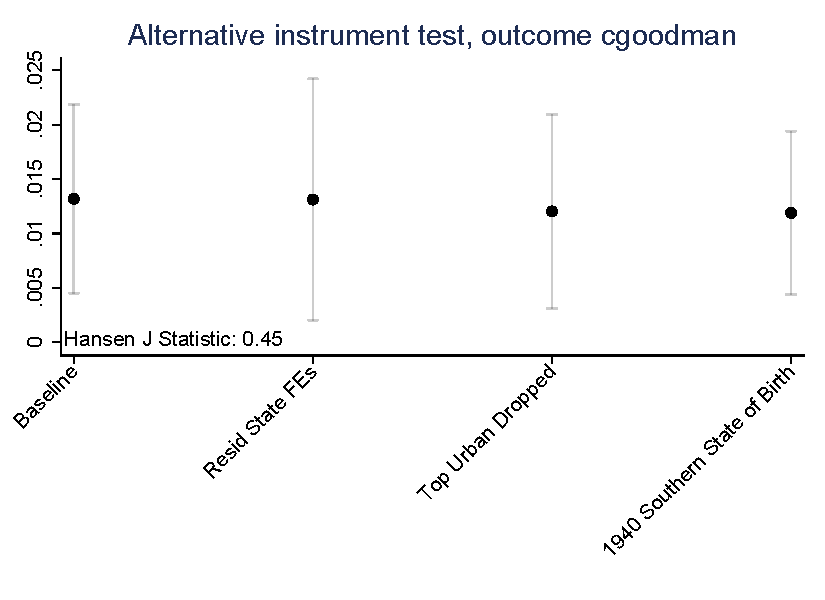
\includegraphics[width=\linewidth]{figures/exogeneity_tests/D16_alt_inst_pooled_cgoodman_new_ctrls.pdf}
        \label{fig:sub1}
    \end{subfigure}
    \begin{subfigure}{0.4\textwidth}
        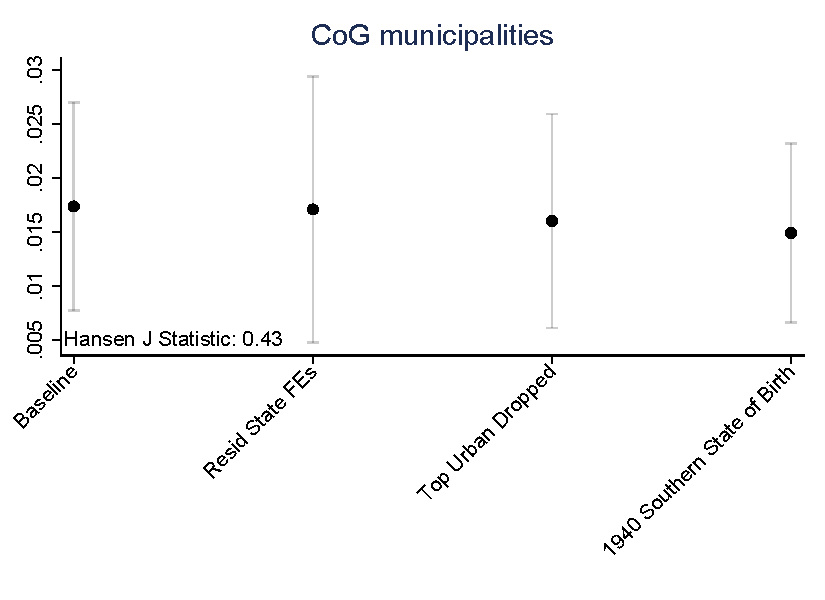
\includegraphics[width=\linewidth]{figures/exogeneity_tests/D16_alt_inst_pooled_gen_muni_new_ctrls.pdf}
        \label{fig:sub2}
    \end{subfigure}
    \begin{subfigure}{0.4\textwidth}
        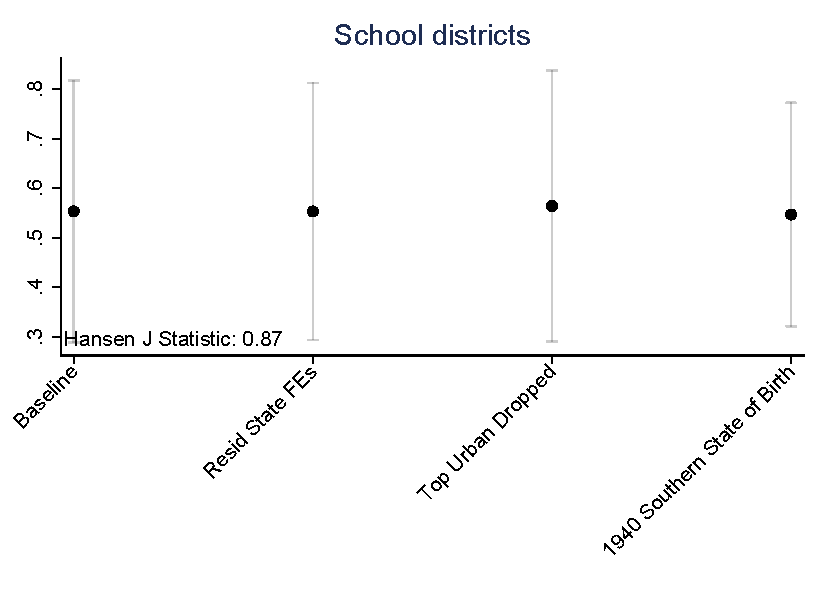
\includegraphics[width=\linewidth]{figures/exogeneity_tests/D16_alt_inst_pooled_schdist_ind_new_ctrls.pdf}
        \label{fig:sub3}
    \end{subfigure}
    \begin{subfigure}{0.4\textwidth}
        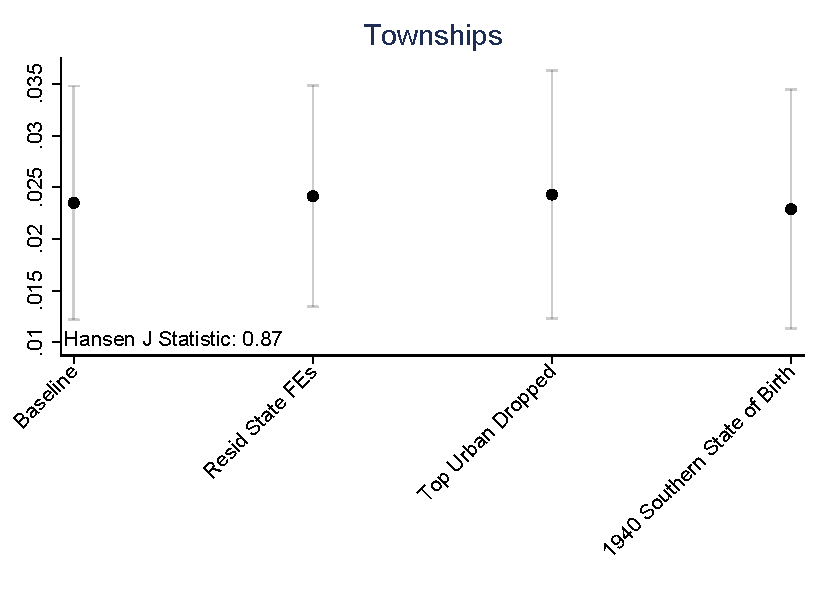
\includegraphics[width=\linewidth]{figures/exogeneity_tests/D16_alt_inst_pooled_gen_town_new_ctrls.pdf}
        \label{fig:sub4}
    \end{subfigure}
    \begin{subfigure}{0.4\textwidth}
        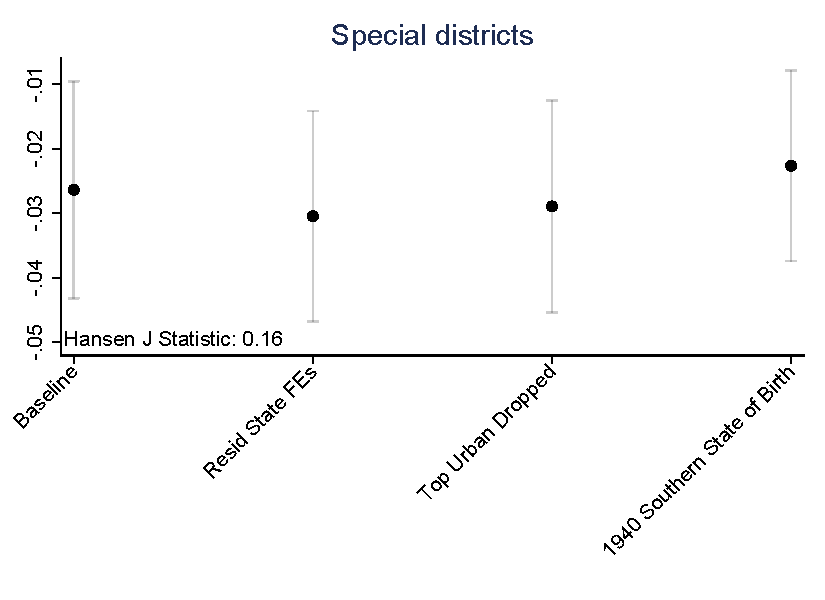
\includegraphics[width=\linewidth]{figures/exogeneity_tests/D16_alt_inst_pooled_spdist_new_ctrls.pdf}
        \label{fig:sub5}
    \end{subfigure}
    \begin{subfigure}{0.4\textwidth}
        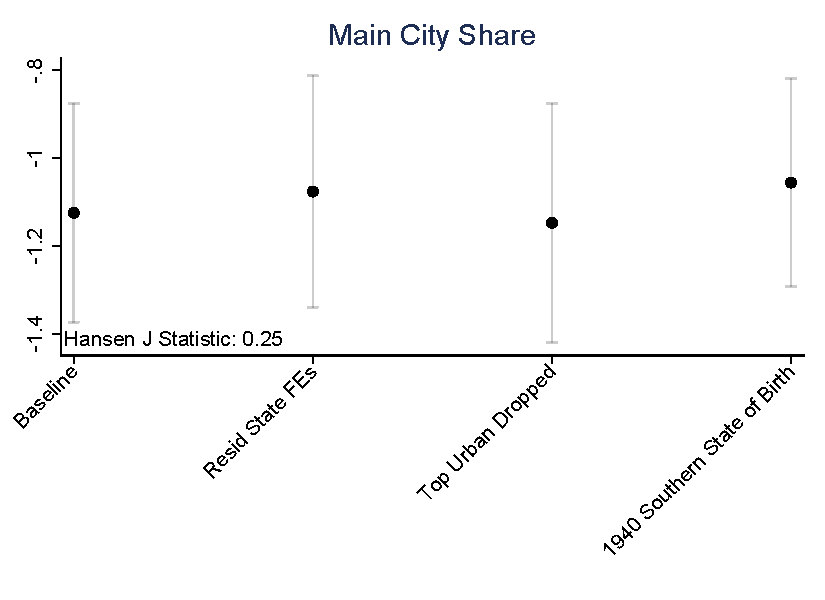
\includegraphics[width=\linewidth]{figures/exogeneity_tests/D16_alt_inst_pooled_totfrac_new_ctrls.pdf}
        \label{fig:sub6}
    \end{subfigure}
    \label{fig:alt_inst}
    \caption*{\scriptsize \emph{Notes:} Point estimates come from our baseline instrument and three alternative instruments, where all specifications include census region fixed effects and CZ-level controls for the sum of shares, coastal, and 1920 transportation cost in 1920, and are weighted by 1940 CZ urban population. Robust standard errors generate 95\% confidence intervals.} 
\end{figure*}

\clearpage


\begin{figure*}[htbp]
    \centering
    \caption{Placebo Tests, Balanced Controls}
    \begin{subfigure}{0.4\textwidth}
        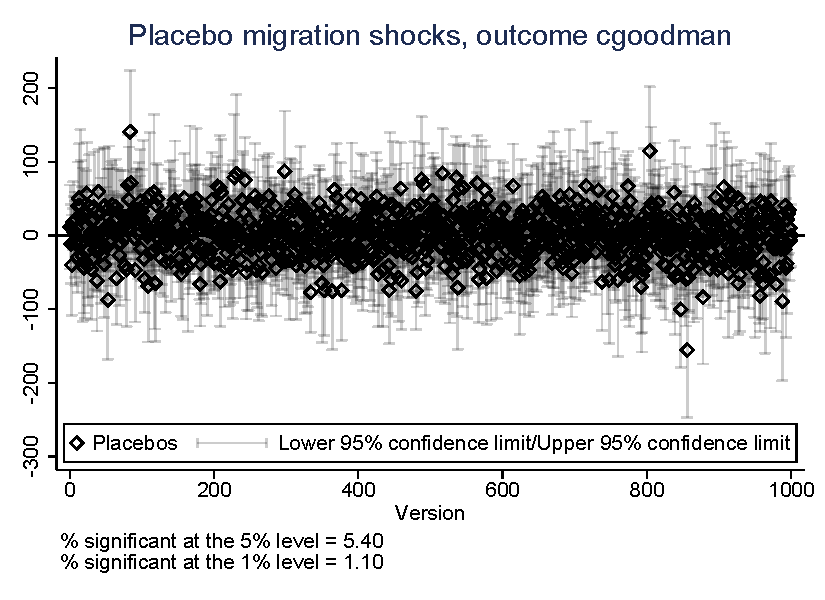
\includegraphics[width=\linewidth]{figures/exogeneity_tests/D17_placebo_cgoodman_new_ctrls.pdf}
        \label{fig:sub1}
    \end{subfigure}
    \begin{subfigure}{0.4\textwidth}
        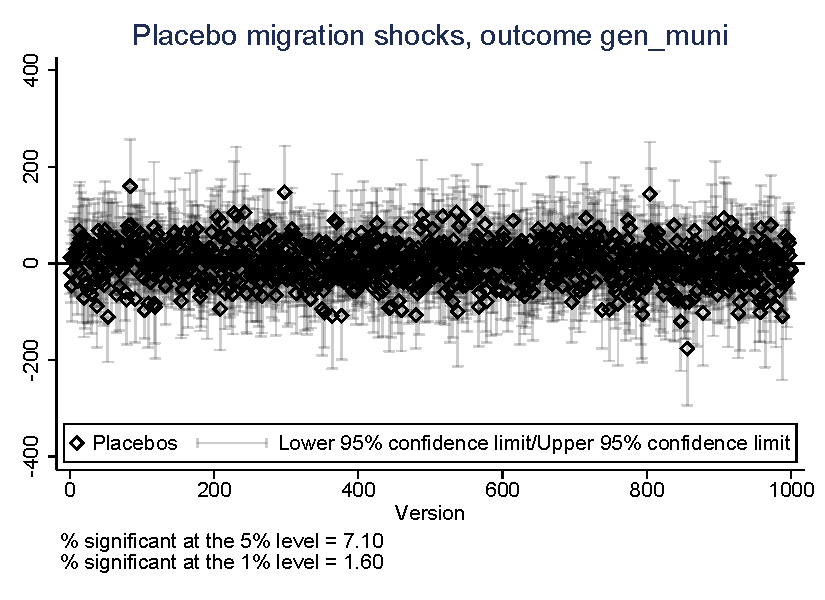
\includegraphics[width=\linewidth]{figures/exogeneity_tests//D17_placebo_gen_muni_new_ctrls.pdf}
        \label{fig:sub2}
    \end{subfigure}
    \begin{subfigure}{0.4\textwidth}
        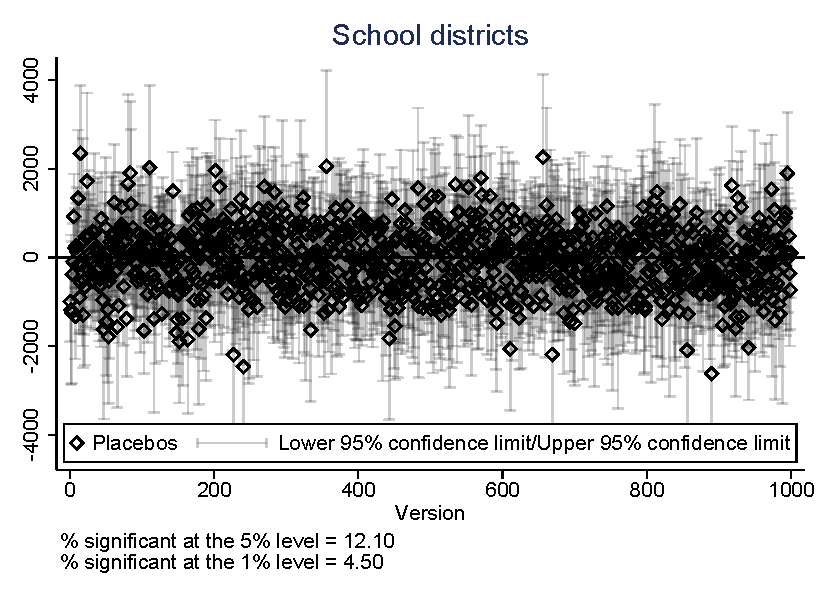
\includegraphics[width=\linewidth]{figures/exogeneity_tests/D17_placebo_schdist_ind_new_ctrls.pdf}
        \label{fig:sub3}
    \end{subfigure}
    \begin{subfigure}{0.4\textwidth}
        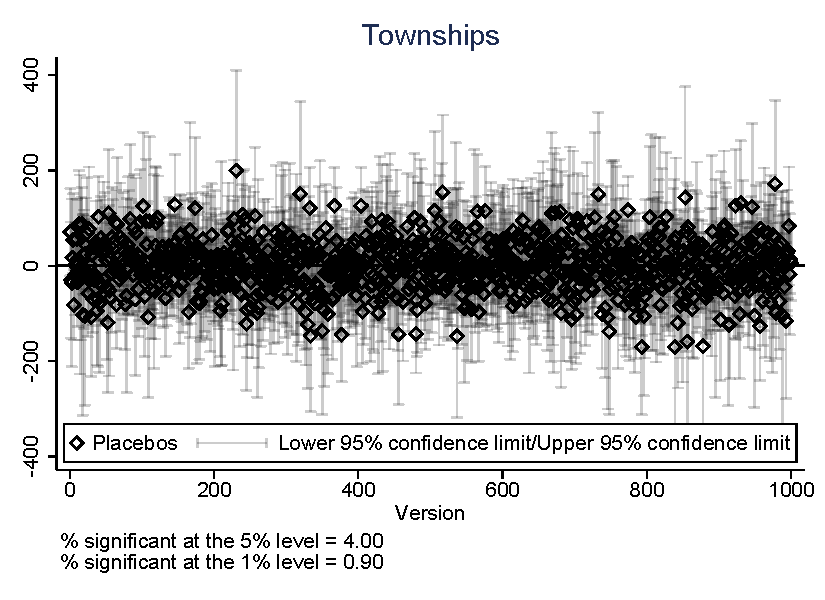
\includegraphics[width=\linewidth]{figures/exogeneity_tests/D17_placebo_gen_town_new_ctrls.pdf}
        \label{fig:sub4}
    \end{subfigure}
    \begin{subfigure}{0.4\textwidth}
        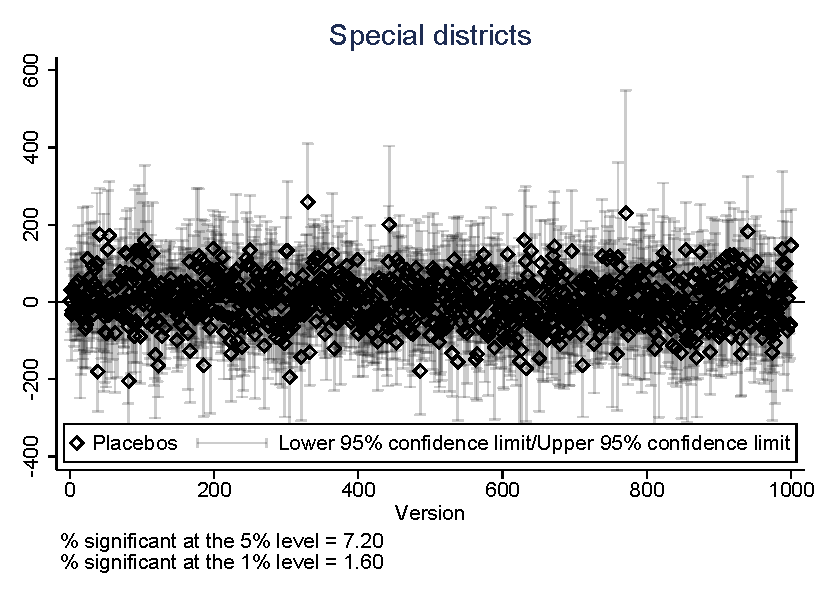
\includegraphics[width=\linewidth]{figures/exogeneity_tests/D17_placebo_spdist_new_ctrls.pdf}
        \label{fig:sub5}
    \end{subfigure}
    \begin{subfigure}{0.4\textwidth}
        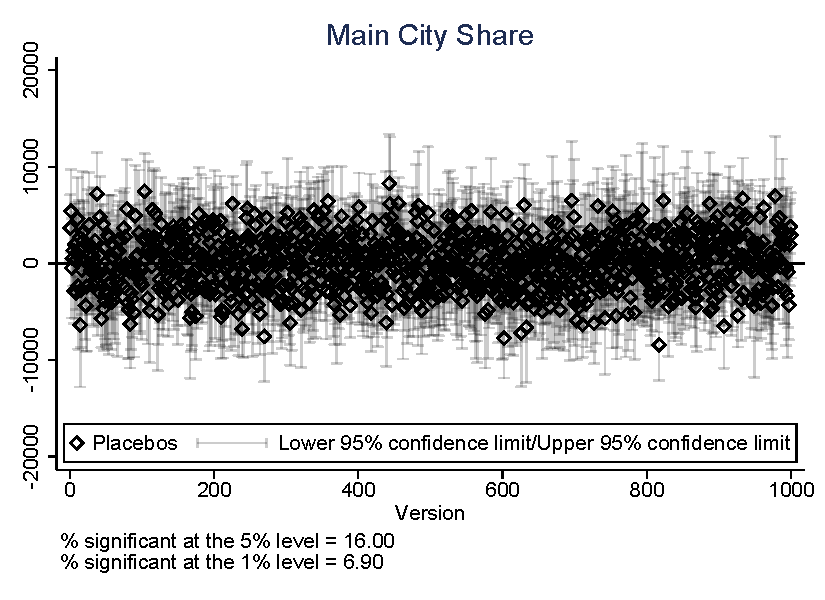
\includegraphics[width=\linewidth]{figures/exogeneity_tests/D17_placebo_totfrac_new_ctrls.pdf}
        \label{fig:sub6}
    \end{subfigure}
    \label{fig:placebo}
    \caption*{\scriptsize \emph{Notes:} Regression results according to equations in the Empirical Strategy section, weighted by 1940 CZ urban population. All specifications include census region fixed effects and CZ-level controls for the sum of shares, coastal, and 1920 transportation cost in 1920. Each of the 1,000 instruments is constructed using randomly generated variation in Southern county-level shocks. Robust standard errors generate 95\% confidence intervals.} 
\end{figure*}


\clearpage
\begin{figure*}[htbp]
    \centering
    \caption{Leave-one-out IV Tests, Balanced Controls}
    \begin{subfigure}{0.4\textwidth}
        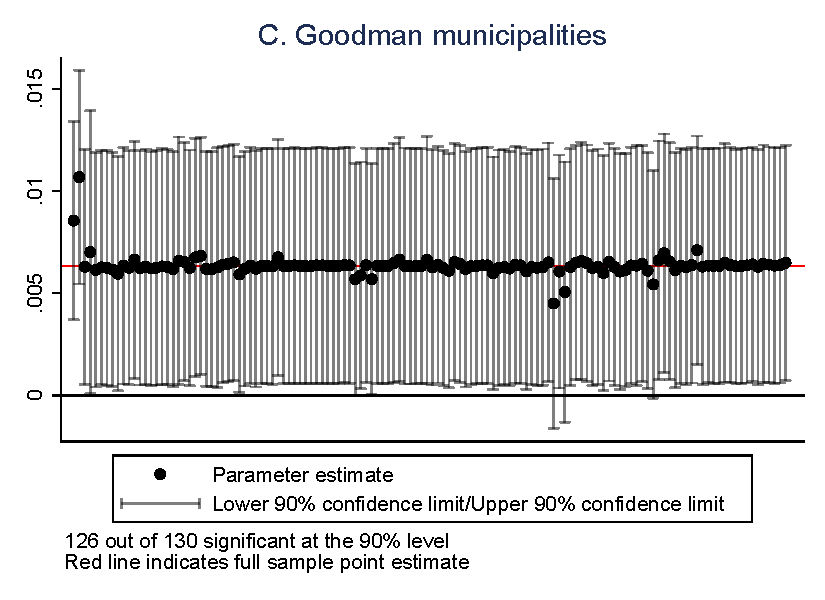
\includegraphics[width=\linewidth]{figures/exogeneity_tests/loo_iv_cgoodman_new_ctrls.pdf}
        \label{fig:sub1}
    \end{subfigure}
    \begin{subfigure}{0.4\textwidth}
        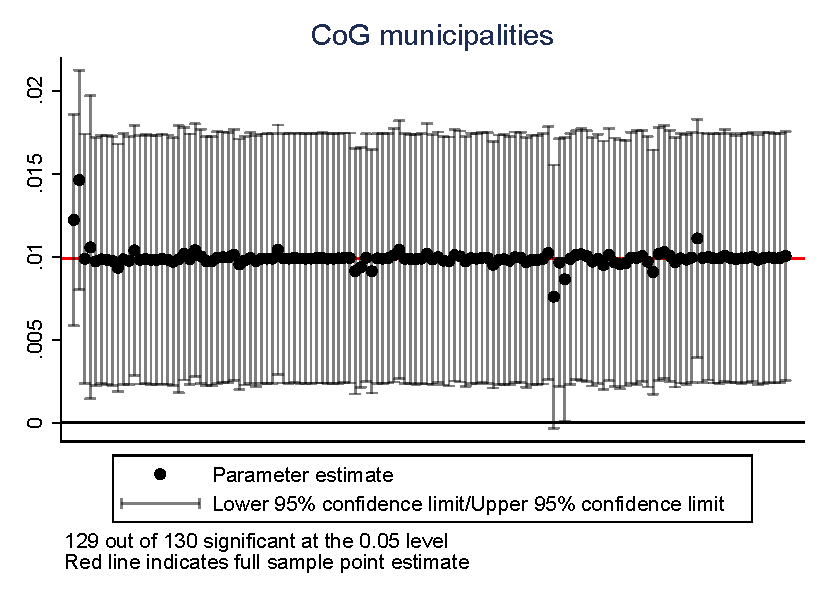
\includegraphics[width=\linewidth]{figures/exogeneity_tests/loo_iv_gen_muni_new_ctrls.pdf}
        \label{fig:sub2}
    \end{subfigure}
    \begin{subfigure}{0.4\textwidth}
        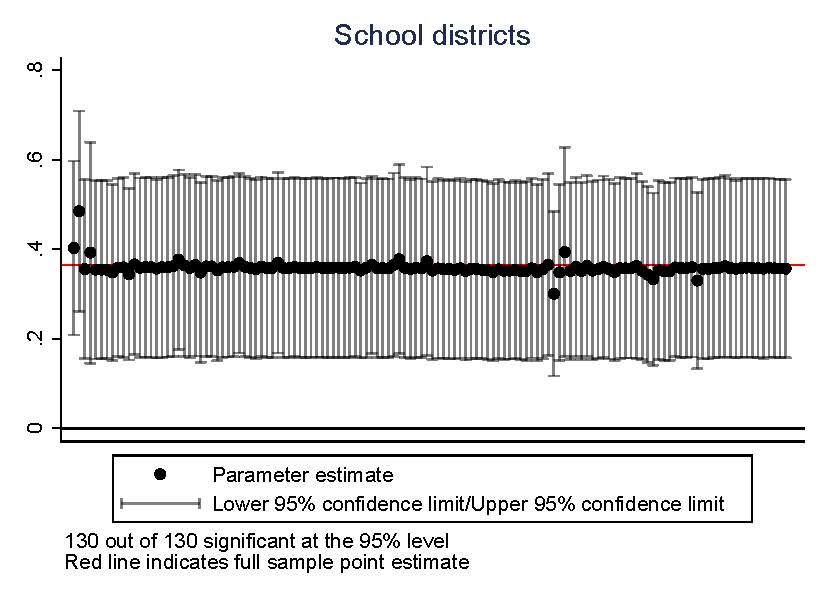
\includegraphics[width=\linewidth]{figures/exogeneity_tests/loo_iv_schdist_ind_new_ctrls.pdf}
        \label{fig:sub3}
    \end{subfigure}
    \begin{subfigure}{0.4\textwidth}
        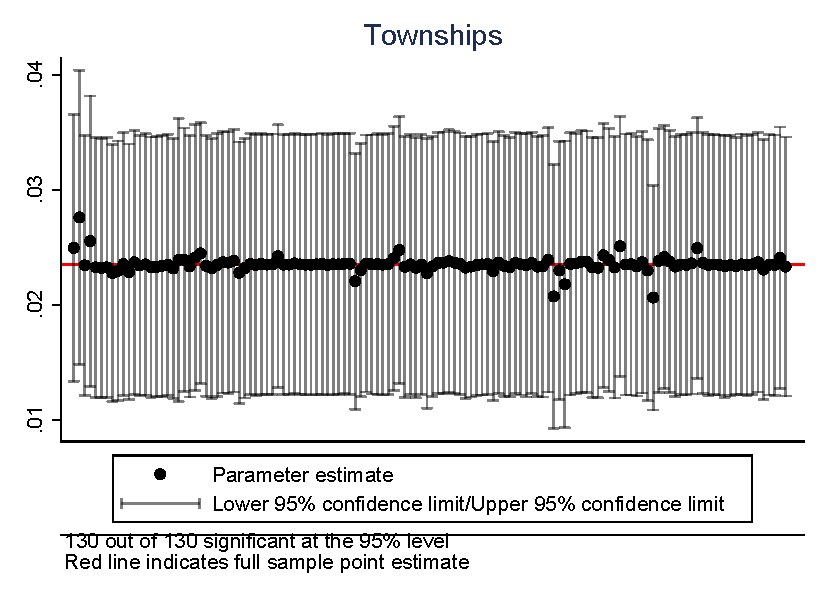
\includegraphics[width=\linewidth]{figures/exogeneity_tests/loo_iv_gen_town_new_ctrls.pdf}
        \label{fig:sub4}
    \end{subfigure}
    \begin{subfigure}{0.4\textwidth}
        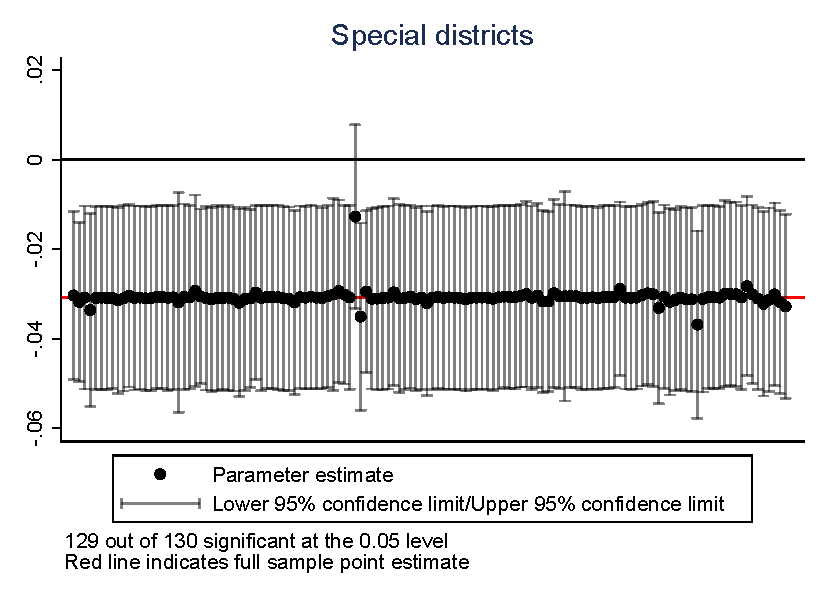
\includegraphics[width=\linewidth]{figures/exogeneity_tests/loo_iv_spdist_new_ctrls.pdf}
        \label{fig:sub5}
    \end{subfigure}
    \begin{subfigure}{0.4\textwidth}
        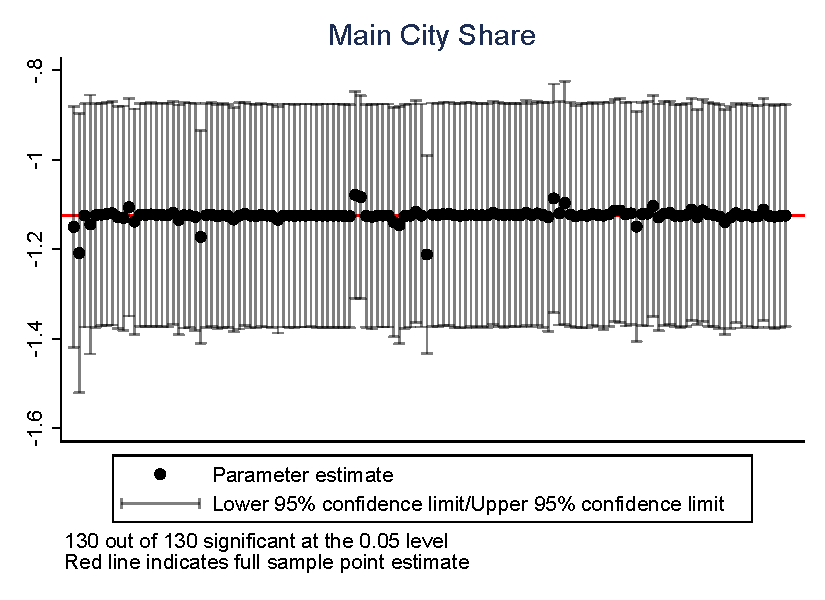
\includegraphics[width=\linewidth]{figures/exogeneity_tests/loo_iv_totfrac_new_ctrls.pdf}
        \label{fig:sub6}
    \end{subfigure}
    \label{fig:loo_iv}
    \caption*{\scriptsize \emph{Notes:} Regression results according to equations in the Empirical Strategy section, weighted by 1940 CZ urban population. All specifications include census region fixed effects and CZ-level controls for the sum of shares, coastal, and 1920 transportation cost in 1920. Each parameter estimate comes from a regression that drops one CZ at a time. Robust standard errors generate 95\% confidence intervals.} 
\end{figure*}
\clearpage
 \begin{tabular}{l*{7}{c}} \toprule
                &\multicolumn{1}{c}{(1)}&\multicolumn{1}{c}{(2)}&\multicolumn{1}{c}{(3)}&\multicolumn{1}{c}{(4)}&\multicolumn{1}{c}{(5)}&\multicolumn{1}{c}{(6)}\\
                &\multicolumn{1}{c}{\shortstack{Variance \\ Ratio}}&\multicolumn{1}{c}{\shortstack{Dissimilarity \\ Index}}&\multicolumn{1}{c}{\shortstack{Relative \\ Concentration}}&\multicolumn{1}{c}{\shortstack{Spatial \\ Proximity}}&\multicolumn{1}{c}{\shortstack{Atkinson \\ Index ($\beta = 0.1$)}}&\multicolumn{1}{c}{\shortstack{Atkinson \\ Index ($\beta = 0.9$)}}\\
\cmidrule(lr){1-7}
\multicolumn{6}{l}{Panel A: IV with GM}\\
\cmidrule(lr){1-7}
GM              &    0.015***&    0.003***&   -0.026   &    0.015***&    0.002***&    0.012***\\
                &  (0.002)   &  (0.001)   &  (0.026)   &  (0.006)   &  (0.000)   &  (0.002)   \\
\cmidrule(lr){1-7}
\multicolumn{6}{l}{Panel B: OLS with $\Delta$ School Districts Per Capita}\\
\cmidrule(lr){1-7}
$\Delta$ School Districts P.C.&    0.012***&    0.003***&   -0.032   &    0.016***&    0.002***&    0.011***\\
                &  (0.002)   &  (0.001)   &  (0.021)   &  (0.004)   &  (0.000)   &  (0.002)   \\
\midrule
Dep. Var. Mean  &    0.092   &    0.192   &   -0.496   &    1.112   &    0.114   &    0.549   \\
Observations    &      118   &      118   &      118   &      118   &      118   &      118   \\
      \bottomrule \end{tabular}

\clearpage
 \begin{tabular}{l*{3}{c}} \toprule
&\multicolumn{1}{c}{Census of Governments}\\\cmidrule(lr){2-2}
&\multicolumn{1}{c}{Townships}\\\cmidrule(lr){2-2}
&\multicolumn{1}{c}{(1)}\\
\cmidrule(lr){1-2}
\multicolumn{1}{l}{Panel A: First Stage}\\
\cmidrule(lr){1-2}
$\widehat{GM}$  &    2.185***\\
                &  (0.302)   \\
\cmidrule(lr){1-2}
\multicolumn{1}{l}{Panel B: OLS}\\
\cmidrule(lr){1-2}
GM              &    0.015***\\
                &  (0.004)   \\
\cmidrule(lr){1-2}
\multicolumn{1}{l}{Panel C: Reduced Form}\\
\cmidrule(lr){1-2}
$\widehat{GM}$  &    0.051***\\
                &  (0.015)   \\
\cmidrule(lr){1-2}
\multicolumn{1}{l}{Panel D: 2SLS}\\
\cmidrule(lr){1-2}
GM              &    0.023***\\
                &  (0.006)   \\
\midrule
First Stage F-Stat&    52.50   \\
Dep. Var. Mean  &    -0.57   \\
1940 Dep. Var. Mean&     2.29   \\
Observations    &      130   \\
 \bottomrule \end{tabular}

\clearpage
\begin{tabular}{l*{7}{c}} \toprule
                &\multicolumn{1}{c}{(1)}   &\multicolumn{1}{c}{(2)}   &\multicolumn{1}{c}{(3)}   &\multicolumn{1}{c}{(4)}   &\multicolumn{1}{c}{(5)}   &\multicolumn{1}{c}{(6)}   \\
&\multicolumn{1}{c}{VR}&\multicolumn{1}{c}{Diss}&\multicolumn{1}{c}{RCO}&\multicolumn{1}{c}{SP}&\multicolumn{1}{c}{Atkinson ($\beta = 0.1$)}&\multicolumn{1}{c}{Atkinson ($\beta = 0.9$)}\\\cmidrule(lr){2-2}\cmidrule(lr){3-3}\cmidrule(lr){4-4}\cmidrule(lr){5-5}\cmidrule(lr){6-6}\cmidrule(lr){7-7}
&\multicolumn{1}{c}{(1)}&\multicolumn{1}{c}{(2)}&\multicolumn{1}{c}{(3)}&\multicolumn{1}{c}{(4)}&\multicolumn{1}{c}{(5)}&\multicolumn{1}{c}{(6)}\\
\cmidrule(lr){1-7}
Percentage Point Change in Urban Black Population&    0.012***&    0.003***&   -0.037*  &    0.016** &    0.002***&    0.012***\\
                &  (0.002)   &  (0.001)   &  (0.023)   &  (0.008)   &  (0.001)   &  (0.003)   \\
\midrule
Dep. Var. Mean  &    0.092   &    0.192   &   -0.496   &    1.112   &    0.080   &    0.340   \\
Observations    &      130   &      130   &      130   &      130   &      130   &      130   \\
       \bottomrule \end{tabular}

\clearpage
 \begin{tabular}{l*{9}{c}} \toprule
                &\multicolumn{2}{c}{\shortstack{Percentage of \\ Municipal Land Uses}}&\multicolumn{3}{c}{\shortstack{Percentage of \\ Municipal Revenues}}&\multicolumn{4}{c}{\shortstack{Percentage of \\ Schools}}\\\cmidrule(lr){2-3}\cmidrule(lr){4-6}\cmidrule(lr){7-10}
                &\multicolumn{1}{c}{(1)}&\multicolumn{1}{c}{(2)}&\multicolumn{1}{c}{(3)}&\multicolumn{1}{c}{(4)}&\multicolumn{1}{c}{(5)}&\multicolumn{1}{c}{(6)}&\multicolumn{1}{c}{(7)}&\multicolumn{1}{c}{(8)}&\multicolumn{1}{c}{(9)}\\
                &\multicolumn{1}{c}{Single Family}&\multicolumn{1}{c}{Apartments}&\multicolumn{1}{c}{Fines/Forfeits}&\multicolumn{1}{c}{\shortstack{Special \\ Assessments}}&\multicolumn{1}{c}{\shortstack{Outstanding \\ Debt}}&\multicolumn{1}{c}{Pct Offering AP}&\multicolumn{1}{c}{Pct Offering DE}&\multicolumn{1}{c}{Mean AP}&\multicolumn{1}{c}{Var AP}\\
\midrule
Above Median GM &   -3.970   &    0.740***&    0.573***&    0.115   &   -8.570   &    0.013   &   -0.032   &    0.632   &   -0.267   \\
                &  (2.959)   &  (0.262)   &  (0.170)   &  (0.428)   & (12.924)   &  (0.036)   &  (0.036)   &  (0.736)   &  (6.056)   \\
\addlinespace
Above Median GM X Inc. 1940-70&   10.699***&   -0.650***&    0.777***&   -1.824***&  -23.954   &    0.183***&    0.115   &    2.464** &  -18.037   \\
                &  (2.713)   &  (0.181)   &  (0.271)   &  (0.615)   & (39.286)   &  (0.057)   &  (0.119)   &  (1.085)   & (14.765)   \\
\addlinespace
Incorporated 1940-70&   -3.240   &   -0.300** &   -0.311   &    1.626***&   11.143   &   -0.169***&   -0.168   &   -1.011*  &   21.890   \\
                &  (2.345)   &  (0.118)   &  (0.193)   &  (0.600)   & (40.730)   &  (0.036)   &  (0.110)   &  (0.572)   & (15.244)   \\
\midrule
Observations    &     7711   &     7711   &     7737   &     7737   &     7737   &     3258   &     3260   &     3258   &     1299   \\
 \bottomrule \end{tabular}

\clearpage
 \begin{tabular}{l*{8}{c}} \toprule
                &\multicolumn{1}{c}{(1)}&\multicolumn{1}{c}{(2)}\\
                &\multicolumn{1}{c}{\shortstack{Adjacent to \\ Principle City}}&\multicolumn{1}{c}{\shortstack{Outstanding Debt as  \\ Pct of Municipal Revenues}}\\
\midrule
Above Median GM X Inc. 1940-70&   -0.046   &  -27.132   \\
                &  (0.144)   & (37.523)   \\
\addlinespace
Above Median GM &    0.005   &  -11.683   \\
                &  (0.038)   & (12.737)   \\
\addlinespace
Incorporated 1940-70&    0.462   &   50.974   \\
                &  (0.280)   &(177.372)   \\
\midrule
Below Median Avg.&    0.250   &  150.680   \\
Observations    &     7719   &     7738   \\
 \bottomrule \end{tabular}

\clearpage
\begin{tabular}{l*{7}{c}} \toprule
&\multicolumn{2}{c}{School District Segregation}&\multicolumn{4}{c}{School District Achievement}\\\cmidrule(lr){2-3}\cmidrule(lr){4-7}
&\multicolumn{1}{c}{\shortstack{Variance \\ Ratio}}&\multicolumn{1}{c}{\shortstack{Dissimilarity \\ Index}}&\multicolumn{1}{c}{\shortstack{Interquartile \\ Range}}&\multicolumn{1}{c}{\shortstack{Variance}}&\multicolumn{1}{c}{\shortstack{Black}}&\multicolumn{1}{c}{\shortstack{White}}\\\cmidrule(lr){2-2}\cmidrule(lr){3-3}\cmidrule(lr){4-4}\cmidrule(lr){5-5}\cmidrule(lr){6-6}\cmidrule(lr){7-7}
&\multicolumn{1}{c}{(1)}&\multicolumn{1}{c}{(2)}&\multicolumn{1}{c}{(3)}&\multicolumn{1}{c}{(4)}&\multicolumn{1}{c}{(5)}&\multicolumn{1}{c}{(6)}\\
\cmidrule(lr){1-7}
\multicolumn{6}{l}{Panel A: First Stage}\\
\cmidrule(lr){1-7}
Predicted Percentage Change in Urban Black Population&    1.341***&    1.341***&    1.341***&    1.341***&    1.341***&    1.341***\\
                &  (0.377)   &  (0.377)   &  (0.377)   &  (0.377)   &  (0.377)   &  (0.377)   \\
\cmidrule(lr){1-7}
\multicolumn{6}{l}{Panel B: OLS}\\
\cmidrule(lr){1-7}
$\Delta\_{1940-70}$ School Districts P.C.&    0.012***&    0.003***&    0.009***&    0.004***&   -0.005** &    0.006***\\
                &  (0.002)   &  (0.001)   &  (0.002)   &  (0.001)   &  (0.002)   &  (0.001)   \\
\cmidrule(lr){1-7}
\multicolumn{6}{l}{Panel C: Reduced Form}\\
\cmidrule(lr){1-7}
Predicted Percentage Change in Urban Black Population&    0.037***&    0.008***&    0.022** &    0.010***&   -0.021** &   -0.021** \\
                &  (0.007)   &  (0.002)   &  (0.010)   &  (0.004)   &  (0.008)   &  (0.008)   \\
\cmidrule(lr){1-7}
\multicolumn{6}{l}{Panel D: 2SLS}\\
\cmidrule(lr){1-7}
$\Delta\_{1940-70}$ School Districts P.C.&    0.027***&    0.006***&    0.016***&    0.008***&   -0.016** &    0.000   \\
                &  (0.005)   &  (0.001)   &  (0.004)   &  (0.001)   &  (0.007)   &  (0.004)   \\
\midrule
First Stage F-Stat&    12.67   &    12.67   &    12.67   &    12.67   &    12.67   &    12.67   \\
Dep. Var. Mean  &     0.21   &     0.26   &     0.32   &     0.07   &    -0.13   &     0.11   \\
Observations    &      118   &      118   &      118   &      118   &      118   &      118   \\
 \bottomrule \end{tabular}

\clearpage
\begin{tabular}{l*{7}{c}} \toprule
&\multicolumn{2}{c}{School District Segregation}&\multicolumn{4}{c}{School District Achievement}\\\cmidrule(lr){2-3}\cmidrule(lr){4-7}
&\multicolumn{1}{c}{\shortstack{Variance \\ Ratio}}&\multicolumn{1}{c}{\shortstack{Dissimilarity \\ Index}}&\multicolumn{1}{c}{\shortstack{Interquartile \\ Range}}&\multicolumn{1}{c}{\shortstack{Variance}}&\multicolumn{1}{c}{\shortstack{Black}}&\multicolumn{1}{c}{\shortstack{White}}\\\cmidrule(lr){2-2}\cmidrule(lr){3-3}\cmidrule(lr){4-4}\cmidrule(lr){5-5}\cmidrule(lr){6-6}\cmidrule(lr){7-7}
&\multicolumn{1}{c}{(1)}&\multicolumn{1}{c}{(2)}&\multicolumn{1}{c}{(3)}&\multicolumn{1}{c}{(4)}&\multicolumn{1}{c}{(5)}&\multicolumn{1}{c}{(6)}\\
\cmidrule(lr){1-7}
\multicolumn{6}{l}{Panel A: First Stage}\\
\cmidrule(lr){1-7}
Predicted Percentage Change in Urban Black Population&    1.377***&    1.377***&    1.377***&    1.377***&    1.377***&    1.377***\\
                &  (0.384)   &  (0.384)   &  (0.384)   &  (0.384)   &  (0.384)   &  (0.384)   \\
\cmidrule(lr){1-7}
\multicolumn{6}{l}{Panel B: OLS}\\
\cmidrule(lr){1-7}
$\Delta\_{1940-2010}$ School Districts P.C.&    0.012***&    0.003***&    0.009***&    0.004***&   -0.005** &    0.006***\\
                &  (0.002)   &  (0.001)   &  (0.002)   &  (0.001)   &  (0.002)   &  (0.001)   \\
\cmidrule(lr){1-7}
\multicolumn{6}{l}{Panel C: Reduced Form}\\
\cmidrule(lr){1-7}
Predicted Percentage Change in Urban Black Population&    0.037***&    0.008***&    0.022** &    0.010***&   -0.021** &   -0.021** \\
                &  (0.007)   &  (0.002)   &  (0.010)   &  (0.004)   &  (0.008)   &  (0.008)   \\
\cmidrule(lr){1-7}
\multicolumn{6}{l}{Panel D: 2SLS}\\
\cmidrule(lr){1-7}
$\Delta\_{1940-2010}$ School Districts P.C.&    0.027***&    0.005***&    0.016***&    0.008***&   -0.015** &    0.000   \\
                &  (0.005)   &  (0.001)   &  (0.004)   &  (0.001)   &  (0.007)   &  (0.004)   \\
\midrule
First Stage F-Stat&    12.88   &    12.88   &    12.88   &    12.88   &    12.88   &    12.88   \\
Dep. Var. Mean  &     0.21   &     0.26   &     0.32   &     0.07   &    -0.13   &     0.11   \\
Observations    &      118   &      118   &      118   &      118   &      118   &      118   \\
 \bottomrule \end{tabular}

\clearpage
\end{landscape}


\begin{figure}
    \centering
    \caption{Most incorporations in 1940-1970 are mostly White}\label{fig:pcarrow_figure}
    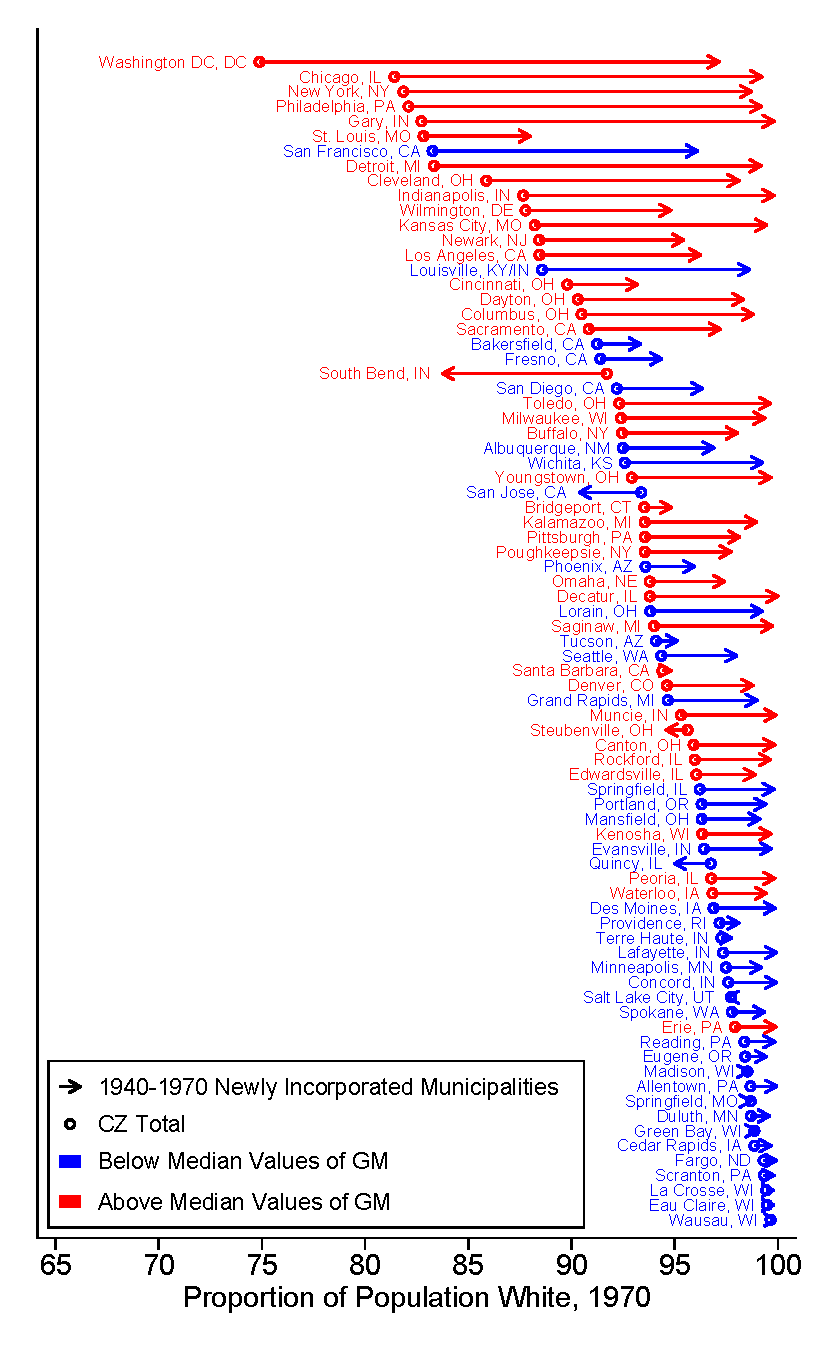
\includegraphics[width = .55\textwidth]{figures/pcarrow_figure_GM_hat.pdf}
    \caption*{\scriptsize \emph{Notes:} Share of White residents in 79 of 130 CZs of our data (those with sub-CZ racial data in 1970), depicted as circles, and the share of White residents in municipalities that were incorporated in 1940-1970, at the tip of the arrows. Some CZs are not shown in this figure because they either had no incorporations or were missing data on racial shares by municipality in those years. Newly incorporated municipalities have a lower share of White residents in only four of the 79 CZs for which we can conduct this exercise.}
\end{figure}

\clearpage



\end{document}
